	\documentclass[10pt,oneside]{CBFT_book}
	
	% Paquetes que cargan
	
	\usepackage{standalone}
	\usepackage{amssymb}
	\usepackage{amsmath}
	\usepackage{graphicx}
	\usepackage{libertine}
	\usepackage[bold-style=TeX]{unicode-math}
	\usepackage{lipsum}

	\usepackage[numbers]{natbib}
	\setcitestyle{square}

	\usepackage{polyglossia}
	\setdefaultlanguage{spanish}
	
	\usepackage{CBFT.estilo} % Cargo la hoja de estilo
	
	\title{CURSO BÁSICO DE FÍSICA TEÓRICA}
	\subtitle{Volumen 2: Física Teórica 1 [Electromagnetismo]}
	\author{E.F. Lavia y Colaboradores}
	\date{\today}
	\version{versión 0.1}

	%###########################################################################
	%		DOCUMENTO 
	%###########################################################################
	
	\begin{document}
	\maketitle	
	
%	\pagenumbering{roman}
	\thispagestyle{empty}
	
	\tableofcontents
	
	\thispagestyle{empty}
	
	
% 	\listoffigures
	
% 	\listoftables

% 	\include{chaps/cft_prefacio}

	\clearpage

	%###########################################################################
	%		CAPITULOS DEL CURSO
	%###########################################################################
	
	\pagenumbering{arabic}
	
		\documentclass[10pt,oneside]{CBFT_book}
	% Algunos paquetes
	\usepackage{amssymb}
	\usepackage{amsmath}
	\usepackage{graphicx}
	\usepackage{libertine}
	\usepackage[bold-style=TeX]{unicode-math}
	\usepackage{lipsum}

	\usepackage{natbib}
	\setcitestyle{square}

	\usepackage{polyglossia}
	\setdefaultlanguage{spanish}


	\usepackage{CBFT.estilo} % Cargo la hoja de estilo

	% Tipografías
	% \setromanfont[Mapping=tex-text]{Linux Libertine O}
	% \setsansfont[Mapping=tex-text]{DejaVu Sans}
	% \setmonofont[Mapping=tex-text]{DejaVu Sans Mono}

	%===================================================================
	%	DOCUMENTO PROPIAMENTE DICHO
	%===================================================================

\begin{document}

% =================================================================================================
\chapter{Conceptos fundamentales de electromagnetismo}
% =================================================================================================

\begin{figure}[htb]
	\begin{center}
	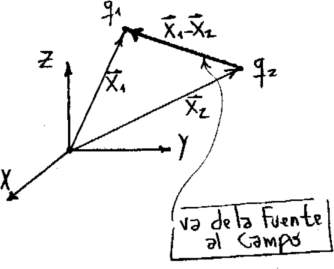
\includegraphics[width=0.6\textwidth]{images/fig_ft1_ejescargas.pdf}	 
	\end{center}
	\caption{}
\end{figure} 


\begin{figure}[htb]
	\begin{center}
	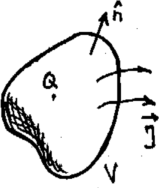
\includegraphics[width=0.6\textwidth]{images/fig_ft1_conserv.pdf}	 
	\end{center}
	\caption{}
\end{figure} 

% =================================================================================================
\section{Ley de Gauss}
% =================================================================================================

\begin{figure}[htb]
	\begin{center}
	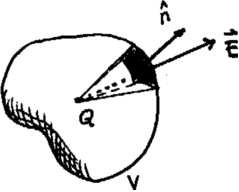
\includegraphics[width=0.6\textwidth]{images/fig_ft1_gauss.pdf}	 
	\end{center}
	\caption{}
\end{figure} 


\begin{figure}[htb]
	\begin{center}
	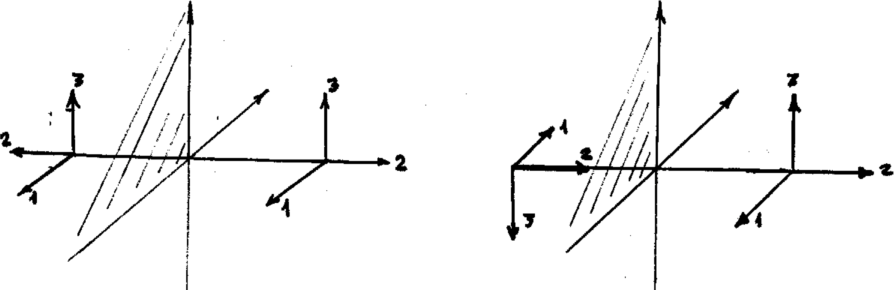
\includegraphics[width=0.6\textwidth]{images/fig_ft1_reflexvect.pdf}	 
	\end{center}
	\caption{}
\end{figure} 

% \bibliographystyle{CBFT-apa-good}	% (uses file "apa-good.bst")
% \bibliography{CBFT.Referencias} % La base de datos bibliográfica

\end{document}

	
		\documentclass[10pt,oneside]{CBFT_book}
	% Algunos paquetes
	\usepackage{amssymb}
	\usepackage{amsmath}
	\usepackage{graphicx}
	\usepackage{bm}
% 	\usepackage{libertine}
	\usepackage[bold-style=TeX]{unicode-math}
	\usepackage{lipsum}

	\usepackage{natbib}
	\setcitestyle{square}

	\usepackage{polyglossia}
	\setdefaultlanguage{spanish}


	\usepackage{CBFT.estilo} % Cargo la hoja de estilo

	% Tipografías
	% \setromanfont[Mapping=tex-text]{Linux Libertine O}
	% \setsansfont[Mapping=tex-text]{DejaVu Sans}
	% \setmonofont[Mapping=tex-text]{DejaVu Sans Mono}

	%===================================================================
	%	DOCUMENTO PROPIAMENTE DICHO
	%===================================================================

\begin{document}

% =================================================================================================
\chapter{Teorema de Green}
% =================================================================================================

% =================================================================================================
\section{Imágenes y método de Green}
% =================================================================================================

El método de las imágenes es un procedimiento gráfico de encontrar problemas equivalentes simulando
con cargas extras (cargas imagen) las condiciones de contorno.

\begin{figure}[htb]
	\begin{center}
	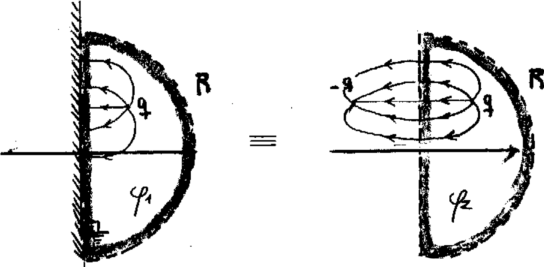
\includegraphics[width=0.6\textwidth]{images/fig_ft1_imagegreen1.pdf}	 
	\end{center}
	\caption{}
\end{figure} 

Los problemas que ilustra la figura satisfacen iguales condiciones de contorno en el recinto punteado,
entonces sus soluciones internas son la misma: $\phi_1 = \phi_2$ por unicidad.

\subsection{El Método de Green}

El concepto tras el método de Green es evaluar el $\phi$ de una carga puntual ante cierta configuración
de contornos conductores. Es una excitación elemental.

Restando entre sí
\[
	\Nabla\cdot(\phi\Nabla\psi) = \phi\lapm{\psi} + \Nabla\phi\cdot\Nabla\psi
\]
y
\[
	\Nabla\cdot(\psi\Nabla\phi) = \psi\lapm{\phi} + \Nabla\psi\cdot\Nabla\phi
\]
e integrando ambos miembros y utilizando el teorema de la divergencia, se llega a
\[
	\int_V \left[ \phi\lapm{\psi} - \psi\lapm{\phi}\right] dV =
	\int_S \left[ \phi\Nabla\psi - \psi\Nabla\phi \right] dS,
\]
que es la segunda identidad de Green.

Consideremos lo que llamaremos caso A, según vemos en figura, caracterizado según
\[
	\rho_{int} \qquad \vb{x}'\in R, \vb{x}\in R
\]
\begin{figure}[htb]
	\begin{center}
	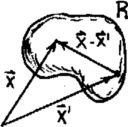
\includegraphics[width=0.2\textwidth]{images/fig_ft1_imagegreen2.pdf}	 
	\end{center}
	\caption{}
\end{figure} 
\[
	\psi = \frac{1}{|\vb{x}-\vb{x}'|} \qquad \lapm{\psi} = -4\pi \delta(\vb{x}-\vb{x}')
\]
\[
	-\phi(\vb{x})4\pi + \int_V 4\pi \frac{\rho(\vb{x}')}{|\vb{x}-\vb{x}'|} \; dV' =
	\int_S \left( \phi\dpar{\psi}{n}-\frac{1}{|\vb{x}-\vb{x}'|}\dpar{\phi}{n}\right)\; dS 
\]
donde estamos usando la abreviatura $\Nabla\phi\cdot\vb{n}=\partial\phi/\partial n$ que es la
derivada normal en la superficie. Despejando
\[
	\phi(\vb{x}) = \int_V \frac{\rho(\vb{x}')}{|\vb{x}-\vb{x}'|} \; dV' +
	\frac{1}{4\pi} \int_S \left( \frac{1}{|\vb{x}-\vb{x}'|}\dpar{\phi}{n} -\phi\frac{\partial}{\partial 
n} \left[\frac{1}{|\vb{x}-\vb{x}'|} \right] \right)\; dS ,
\]
donde la primer integral es debido a las cargas internas y la segunda al efecto de las cargas
fuera del reciento $R$.

Recordemos que las condiciones tipo Dirichlet corresponden a $\phi|_S$ y las tipo Neumann a
$\partial\phi/\partial \hat{n}|_S$.

El caso B, según figura, corresponde a
\[
	\rho_{int} \qquad \vb{x}'\notin R, \vb{x}\in R
\]
y 
\[
	\int_V \frac{\rho(\vb{x}')}{|\vb{x}-\vb{x}'|} \; dV' = 
	\frac{1}{4\pi} \int_S \left( \phi\frac{\partial}{\partial n} \left[\frac{1}{|\vb{x}-\vb{x}'|} \right]
	- \frac{1}{|\vb{x}-\vb{x}'|}\dpar{\phi}{n}  \right)\; dS ,
\]
la integral de superficie proviene de las cargas fuera de $R$ que producen campo en el interior
$R$.

\begin{figure}[htb]
	\begin{center}
	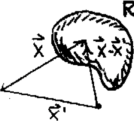
\includegraphics[width=0.2\textwidth]{images/fig_ft1_imagegreen3.pdf}	 
	\end{center}
	\caption{}
\end{figure} 

Hemos tomado $\psi=1/|\vb{x}-\vb{x}'|$ que verifica [1]; interpretándose $\psi$ como el potencial
de una carga puntual unitaria.

\[
	\lapm{\frac{1}{|\vb{x}-\vb{x}'|}} = - 4\pi \delta( |\vb{x}-\vb{x}'| )
\]
podemos tomar
\[
	G \equiv \frac{1}{|\vb{x}-\vb{x}'|} + f( \vb{x}, \vb{x}')
\]
donde $G$ es la función de Green.

\[
	\lapm{G} = -4\pi  \delta( \vb{x}, \vb{x}' ) + \lapm{f}
\]
donde $F$ satisface Laplace (si el reciento no incluye a $\vb{x}'$).
Con $\lapm{f( \vb{x}, \vb{x}' )}$.

Entonces $f( \vb{x}, \vb{x}' )$ representan la o las imágenes necesarias para que
$G$ cumpla el contorno necesario $G_D|_S=0$.


% =================================================================================================
\section{Funciones de Green}
% =================================================================================================

\be
	\phi(\vb{x}) = \int_{V'} G(\vb{x},\vb{x}') \rho(\vb{x}')  \; dV' +
	\frac{1}{4\pi} \int_{S'} \left( G(\vb{x},\vb{x}')\dpar{\phi}{n} -\phi\frac{\partial}{\partial 
	n} G(\vb{x},\vb{x}') \right)\; dS' ,
	\label{green1}
\ee
Pero para poder utilizar \eqref{green1} necesito tener un solo tipo de condiciones de contorno,
de manera que según sean
\[
	\textrm{Dirichlet} \quad 	\begin{cases}
				G_D : \lapm{G_D} = -4\pi \delta(\vb{x},\vb{x}') \\
				G_D |_{contorno de R} = 0  \\
				\phi|_S \\
				\phi(\vb{x}) = \displaystyle \int_{V'} G_D \rho \; dV' - \frac{1}{4\pi}
				\int_{S} \phi|_S\frac{\partial}{\partial n} G_D \; dS'
			\end{cases}
\]
donde la condición de contorno de $G$ equivale, en el contexto físico del electromagnetismo, a
reemplazar el contorno por un conductor metálico puesto a tierra.
Entonces $G$ es el potencial de la configuración de conductores con el contorno puesto a tierra
frente a una carga puntual con magnitud unitaria.

La función de Green da la geometría del problema.

\[
	\dpar{\phi_1}{n}|_S - \dpar{\phi_2}{n}|_S = -4\pi\sigma \qquad \qquad \phi_2|_S = \phi_1|_S
\]

\[
	\textrm{Neumann} \quad 	\begin{cases}
				G_N : \lapm{G_N} = -4\pi \delta(\vb{x},\vb{x}') \\
				\Nabla G_N \cdot \hat{n}|_S = -\frac{4\pi}{S}  \\
				\left.\dpar{\phi}{n}\right|_S \\
				\phi(\vb{x}) = \displaystyle <\phi>|_S + \int_{V'} G_N \rho \; dV' + 
				\frac{1}{4\pi} \int_{S} G_N|_S \dpar{G_N}{n} \; dS
			\end{cases}
\]

\subsection{Green para el problema externo de una esfera}

En este problema las condiciones adecuadas son las de Dirichlet, ver Figura
\begin{figure}[htb]
	\begin{center}
	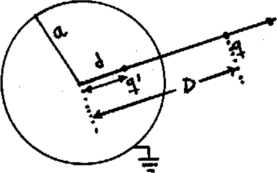
\includegraphics[width=0.4\textwidth]{images/fig_ft1_green1.pdf}	 
	\end{center}
	\caption{}
\end{figure} 
y podemos escribir la función de Green como 
\[
	G = \frac{1}{|\vb{r} - D\hat{r}'|} - \frac{a/D}{|\vb{r} - a^2/D\hat{r}'|} \qquad G|_{r=a}
\]
sujeta a que 
\[
	q' = -q a/D \qquad d = a^2/D
\]
\begin{figure}[htb]
	\begin{center}
	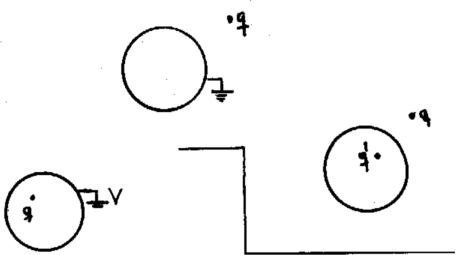
\includegraphics[width=0.6\textwidth]{images/fig_ft1_green2.pdf}	 
	\end{center}
	\caption{$G_D$ es el potencial de la configuración (a) y se evalúa teniendo en cuenta la
	otra (b) que se resuelve casualmente por imágenes. La (c) se resuelve alterando las condiciones.}
\end{figure} 

El caso (c) de la Figura se resuelve con 
\[
	-\frac{V}{4\pi} \int_S \dpar{G}{n} dS = -\frac{V}{4\pi} \int_S \Nabla G\cdot d\vb{S} =
	-\frac{V}{4\pi} \int_V \lapm{G} \: dV	
\]
\[
	= -\frac{V}{4\pi} (-4\pi)\int_V \delta(\vb{x}-\vb{x}') \: dV	= V 
\]

\section{Algunos campos}

En distribuciones infinitas de carga la integral de Poisson diverge pero ello se debe a que en
realidad no existen distribuciones infinitas de carga.
\begin{figure}[thb]
	\begin{center}
	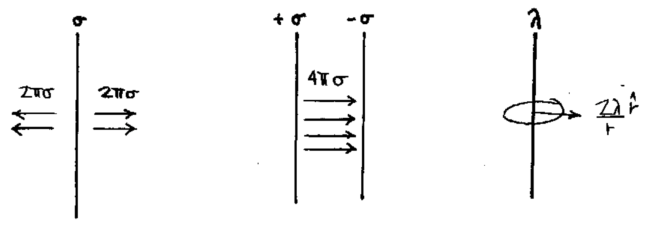
\includegraphics[width=0.8\textwidth]{images/fig_ft1_campohilos.pdf}	 
	\end{center}
	\caption{}
\end{figure} 

\section{Notas método de Green}

Función de Green libre (sin contornos) lleva directo a la integral de Poisson
\[
	G(\vb{x}, \vb{x}') = \frac{1}{|\vb{x} - \vb{x}'|}
\]
entonces 
\[
	\phi(\vb{x}) = \int_V \rho \:G \:dV = \int_{V'} \frac{ \rho(\vb{x}) }{|\vb{x}-\vb{x}'|} dV'
\]
\[
	\nabla^2 \left( \frac{1}{|\vb{x} - \vb{x}'|} \right) = 4\pi \delta(\vb{x}-\vb{x}')
\]
\[
	G(\vb{x}, \vb{x}') =  \frac{1}{|\vb{x} - \vb{x}'|} + f(\vb{x}, \vb{x}') \qquad 
	\textrm{con} \quad \lapm{f}(\vb{x}, \vb{x}') = 0 \quad \textrm{si} \quad \vb{x}\neq\vb{x}'
\]

Para condiciones de Neumann se toma:
\[
	\Nabla G_N|_S = -\frac{4\pi}{S} = \left. \dpar{G}{n} \right|_S
\]
la integral 
\[
	- \frac{1}{4\pi} \int_S \phi|_S \left.\dpar{G}{n}\right|_S  dS
\]
no se puede anular con 
\[
	\left.\dpar{G}{n}\right|_S = 0
\]
salvo que el volumen de integración no contenga a $\vb{x}=\vb{x}'$ en cuyo caso:
se excluye $\vb{x}=\vb{x}'$ de la integración.
\[
	- \frac{1}{4\pi} \int_S \phi|_S \left.\dpar{G}{n}\right|_S  dS =
	\frac{1}{S} \int_S \phi|_S dS = <\phi>|_S
\]
que es el valor promedio de $\phi$ en la superficie $S$.

Se suele tomar la superficie $S \to \infty$ de modo que resulte nulo $<\phi>|_S$.
Se toma el volumen $V$ rodeado por dos superficies una cerrada y finita y la otra
en infinito entonces
\[
	<\phi>|_S = 0 \qquad \qquad \left. \dpar{G}{n}\right|_S = 0
\]
esto es el llamado {\it problema exterior}.

% =================================================================================================
\section{Condiciones de contorno}
% =================================================================================================

La ley de Gauss nos dice
\[
	\int \vb{E} \cdot d\vb{S} = 4 \pi Q_n
\]
para el cilindrito de la figura
\[
	( \vb{E}_2 - \vb{E}_1 )\cdot \hat{n} \Delta S = 4 \pi \sigma \Delta S 
\]
\[
	( \vb{E}_2 - \vb{E}_1 )\cdot \hat{n} = 4 \pi \sigma 
\]
\[
	\rotorm{E} = 0 \Rightarrow \int_\Gamma \vb{E} \cdot d\vb{\ell} = 0 =
	( \vb{E}_2 - \vb{E}_1 )\cdot d\vb{\ell}  = ( \vb{E}_1 + \vb{E}_2 ) \cdot \hat{n}\times\hat{\eta} d\ell
\]
donde esto vale en electrostática (nula la integral de línea del campo \vb{E}) y además
\[
	\hat{n}\times\hat{\eta} = \frac{d\vb{\ell}}{d\ell} 
\]

\begin{figure}[htb]
	\begin{center}
	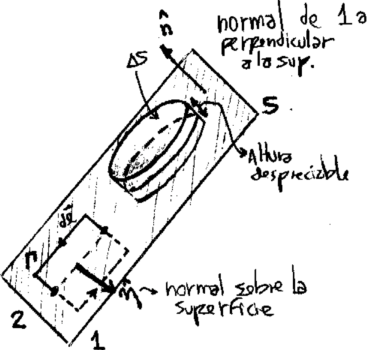
\includegraphics[width=0.4\textwidth]{images/fig_ft1_contorno1.pdf}	 
	\end{center}
	\caption{}
\end{figure} 
y puesto que vale la permutación
\[
	0 = ( -\vb{E}_2 + \vb{E}_1 )\cdot(\hat{n}\times\hat{\eta}) \longrightarrow 
	0 = \hat{\eta} \cdot ( ( -\vb{E}_2 + \vb{E}_1 ) \times \hat{n} )
\]

de modo que la componente tangencial es continua y entonces
\[
	\hat{n} \times ( \vb{E}_2 - \vb{E}_1 ) = 0
\]
\[
	E_{2\hat{n}} - E_{1\hat{n}} = 4 \pi \sigma \qquad \qquad E_{2\hat{t}} -E_{1\hat{t}} = 0
\]
\[
	-\Nabla\phi_2\cdot\hat{n} + \Nabla\phi_1\cdot\hat{n} = 4 \pi \sigma
\]
\[
	\frac{\Nabla(\phi_2-\phi_1)\cdot \hat{n}}{4 \pi} = \sigma
\]
\[
	\sigma = \frac{1}{4\pi}\dpar{(\phi_1-\phi_2)}{n}
\]
esta es la densidad de carga inducida sobre la frontera entre medios.

Para los medios magnéticos
\[
	\rotorm{H} = \frac{4 \pi}{c} \vb{J}_l
\]
\[
	\int_S (\rotorm{H}) \cdot d\vb{S} = \int_S \frac{4 \pi}{c} \vb{J}_l \cdot d\vb{S} = 
	\frac{4 \pi}{C} \vb{g}_l\cdot \hat{s} d\ell
\]
donde hicimos la transformación
\[
	\int \vb{H}\cdot d\ell = (\vb{H}_2-\vb{H}_1)\cdot d\ell
\]
y donde recordemos que la altura de $\Gamma$ tiene a cero.
\[
	\frac{4 \pi}{c} \vb{g}_l \cdot \vb{s} = ( -\vb{H}_2 + \vb{H}_1 )\cdot( \hat{n} \times \hat{s} ) d\ell
\]
\[
	\frac{4 \pi}{c} \vb{g}_l \cdot \vb{s} \; d\ell = (\vb{H}_1 -\vb{H}_2 \times \hat{n})\cdot \hat{s} 
d\ell
\]

\begin{figure}[htb]
	\begin{center}
	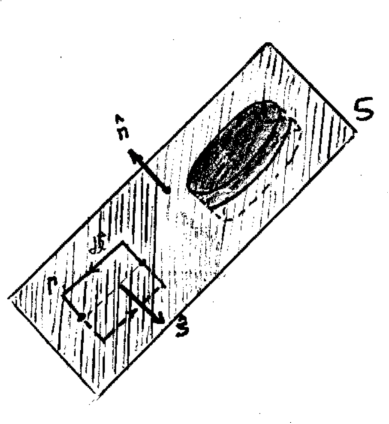
\includegraphics[width=0.4\textwidth]{images/fig_ft1_contorno2.pdf}	 
	\end{center}
	\caption{}
\end{figure} 

de manera que 
\[
	\frac{4 \pi}{c} \vb{g}_l = \hat{n} \times ( \vb{H}_2 - \vb{H}_1 )
\]
\[
	\hat{n}\times\hat{s} = \frac{d\vb{\ell}}{d\ell} 
\]
\[
	B_{2\hat{n}} - B_{1\hat{n}} = 0 \qquad \qquad H_{2\hat{t}} - H_{1\hat{t}} = \frac{4 \pi}{c} g_l
\]
\[
	\int_S \vb{B}\cdot d\vb{S} = 0 \Rightarrow (\vb{B}_2 - \vb{B}_1 )\cdot\hat{n} = 0
\]

% =================================================================================================
\section{Desarrollo multipolar}
% =================================================================================================

\[
	\phi(\vb{x}) = \int_{V'} \frac{\rho(\v{x})}{|\vb{x}-\vb{x}'|} \; dV'
\]
Cuando la expresión es muy complicada podemos desarrollarla en una serie de potencias
\[
	\phi(\vb{x}) = \frac{Q}{|\vb{x}|} + \frac{\vb{x}\cdot\vb{p}}{|\vb{x}|^3} +
	\sum_{i,j}^3 \frac{1}{2|\vb{x}|^5} x_i Q_{ij} x_j
\]
donde está centrado en el origen de coordenadas.

% \bibliographystyle{CBFT-apa-good}	% (uses file "apa-good.bst")
% \bibliography{CBFT.Referencias} % La base de datos bibliográfica

\end{document}

	
		\documentclass[10pt,oneside]{CBFT_book}
	% Algunos paquetes
	\usepackage{amssymb}
	\usepackage{amsmath}
	\usepackage{graphicx}
	\usepackage{libertine}
	\usepackage[bold-style=TeX]{unicode-math}
	\usepackage{lipsum}

	\usepackage{natbib}
	\setcitestyle{square}

	\usepackage{polyglossia}
	\setdefaultlanguage{spanish}


	\usepackage{CBFT.estilo} % Cargo la hoja de estilo

	% Tipografías
	% \setromanfont[Mapping=tex-text]{Linux Libertine O}
	% \setsansfont[Mapping=tex-text]{DejaVu Sans}
	% \setmonofont[Mapping=tex-text]{DejaVu Sans Mono}

	%===================================================================
	%	DOCUMENTO PROPIAMENTE DICHO
	%===================================================================

\begin{document}

% =================================================================================================
\chapter{Método de separación de variables}
% =================================================================================================

% =================================================================================================
\section{Separación de variables}
% =================================================================================================

Separamos los problemas en regiones donde vale $\lapm{\phi} = 0$ entonces las fronteras tendrán la
$\rho(\vb{x}')$ en general en forma de $\sigma,\lambda$.

Para coordenadas cartesianas intentaremos resolver $\lapm{\phi} = 0$, es decir
\[
	\dpar[2]{\phi}{x} + \dpar[2]{\phi}{y}  + \dpar[2]{\phi}{z}  = 0
\]
pidiendo
\[
	\phi(x,y,z) = X(x)Y(y)Z(z)
\]
de manera que 
\[
	\frac{1}{X}\dtot[2]{X}{x} + \frac{1}{Y}\dtot[2]{Y}{y} + \frac{1}{Z}\dtot[2]{Z}{z} = 0 \qquad 
	- \alpha^2  - \beta^2 + \gamma^2 = 0 \quad \Rightarrow  \gamma^2 = \alpha^2 + \beta^2 
\]
cada término es una constante. La solución general es
\[
	\phi(x,y,z) = \sum_{m=0}^\infty \sum_{n=0}^\infty A_{m,n} \euler^{\pm i\alpha_m x}
	\euler^{\pm i\beta_n y} \euler^{\pm i\sqrt{\alpha_m^2 + \beta_n^2 }z}
\]
donde habrá que adaptar según las condiciones de contorno. Se da que $A_{m,n}$ es una constante general
y hay condiciones periódicas en $x,y$
\[
	A\euler^{\pm i\alpha x} = A_\alpha \cos(\alpha x) + B_\alpha \sin(\alpha x)
\]
corresponde a condiciones de potencial periódicas, cuando necesito dos ceros por ejemplo (ver ilustración
lateral --que falta--)
\[
	A\euler^{\pm \gamma z} = A_\gamma \cosh(\gamma z) + B_\gamma \sinh(\gamma z)
\]
corresponde a atravesar densidades de carga.

Para coordenadas esféricas es
\[
	\frac{1}{r} \frac{\partial}{\partial r}\left( r^2 \dpar{\phi}{r} \right) + 
	\frac{1}{r^2 \sin(\theta)}\frac{\partial}{\partial\theta}\left(\sin(\theta)\dpar{\phi}{\theta}\right)+
	\frac{1}{r^2 \sin(\theta)} \dpar[2]{\phi}{\varphi} = 0
\]
proponiéndose la separación
\[
	\phi(r,\theta,\varphi) = R(r) \Theta(\theta) Q(\varphi)
\]
siendo
\[
	Y(\theta,\varphi) = \Theta(\theta) Q(\varphi)
\]
un armónico esférico.
Tenemos un oscilador armónico en $\varphi$,
\[
	Q = \euler^{\pm i\alpha \varphi}
\]
si usamos $0\leq \varphi \leq 2\pi$ de modo que $\alpha\in\mathbb{Z}$ y entonces $\alpha=m$, con simetría
azimutal es $m=0$ (rotación en $\varphi$), 
\[
	Q = G\varphi + H \qquad\qquad  G,H \quad ctes.
\]
Para las otras funciones será
\[
	R(r) = A_\ell r^\ell + B_\ell R^{-\ell-1}
\]
\[
	\Theta(\theta) = C_\ell P_\ell^m (\cos(\theta)) + D_\ell Q_\ell^m (\cos(\theta))
\]
siendo $P_\ell^m$ polinomio de Legendre, que verifica la fórmula de Rodrigues
\[
	P_\ell (x) = \frac{1}{2^\ell \ell!} \frac{d^\ell}{d x^\ell} [x^2 - 1]^\ell
\]
con $P_\ell(\cos(\theta))$ polinomio de Legendre de primera especie, y $Q_\ell(\cos(\theta))$ de segunda
especie.
Los $\{ P_\ell\}$ son un conjunto completo y ortogonal en $-1 \leq x \leq 1$ o bien en $0\leq \theta\leq \pi$.

Los $\{ Q_\ell^m(\cos(\theta))\}$ tienen problemas en $\theta=0,\theta=\pi$ (eje $z$) de manera que si está el
eje $z$ no podemos usar $Q_\ell^m$; en estos problemas sólo podemos usar $P_\ell^m(\cos(\theta))$.
\[
	\phi(r,\theta,\phi) = \sum_{\ell=0}^{\infty}\sum_{m=-\infty}^{\infty} \left[ A_\ell r^\ell + 
	B_\ell r^{-\ell-1} \right] \left[ C_\ell P_\ell^m + D_\ell Q_\ell^m \right] \left[ E_m \cos(m\phi) + 
	F_m \sin(m\phi) \right]
\]
y en el caso particular $m=0$
\[
	\phi(r,\theta,\phi) = \sum_{\ell=0}^{\infty}\sum_{m=-\infty}^{\infty} \left[ A_\ell r^\ell + 
	B_\ell r^{-\ell-1} \right] \left[ C_\ell P_\ell^m + D_\ell Q_\ell^m \right] \left[ G_0 \phi + 
	H_0 \right]	
\]
Las constantes $A_\ell, B_\ell, C_\ell, D_\ell, E_m, F_m$ se ajustan con el $\phi (r\to\infty)$, 
$\phi (r\to 0)$, $\phi (z = 1)$ y $\phi (z = -1)$.

Lo que permite esquivar el problema del punto singular en $x \equiv \cos(\theta)=1$ es
\[
	\beta^2 = \ell(\ell + 1) \qquad - \ell < m < \ell \qquad \alpha^2 = m^2
\]

Recordemos las sumas de series
\[
	\frac{1}{1-z} = \sum_{\ell=0}^{\infty} z^\ell \qquad \frac{1}{1+z} = \sum_{\ell=0}^{\infty} (-1)^\ell 
	z^\ell	\qquad |z|<1,
\]
el polinomio asociado de Legendre
\[
	P_\ell^m (x) =) \frac{(-1)^m}{2^\ell \ell!} [1-x^2]^{m/2} \frac{d^{\ell + m}}{dx^{\ell + m}} 
			[x^2 -1]^\ell
\]
que cumple
\[
	P_\ell (1) = 1 \quad P_\ell (-1) = (-1)^\ell \qquad  \forall \ell
\]
con 
\[
	\int_{-1}^1 [P_\ell (x)]^2 \: dx = \frac{2}{ 2\ell + 1 }
\]
siendo la ortogonalidad
\[
	\int_0^\pi P_{\ell'}^m (\cos(\theta)) P_\ell^m (\cos(\theta)) \sin(\theta) \: d\theta = 
	\delta_{\ell\ell'}
\]
\[
	\int_{-1}^{+1} P_{\ell'}^m (x) P_\ell^m (x) \: dx= \frac{2}{2\ell + 1}
	\frac{(\ell + m)!}{(\ell - m)!} \: \delta_{\ell\ell'}
\]

En esféricas las constantes de separación están asociadas
\[
	R(r) \; \mathrm{con} \; \ell \qquad \Theta(\theta) \; \mathrm{con} \; \ell,m \qquad
	Q(\phi) \; \mathrm{con} \; m
\]

% =================================================================================================
\section{Detalles sobre solución de problemas de potencial}
% =================================================================================================

Si el potencial es par en una coordenada, entonces uso funciones pares (cosenos). 
La continuidad del potencial
\[
	\phi_I(x=0) = \phi_{II}(x=0) = 
\]
y salto en el campo
\[
	\left.\dpar{\phi_I}{x} - \dpar{\phi_{II}}{x}\right|_{x=0} = -4\pi\sigma|_{x=0}
\]

\begin{figure}[htb]
	\begin{center}
	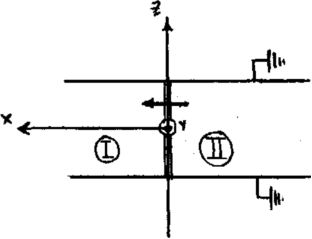
\includegraphics[width=0.4\textwidth]{images/fig_ft1_potencial.pdf}	 
	\end{center}
	\caption{}
\end{figure} 
Si tengo condiciones periódicas en la coordenada irán senos y cosenos trigonométricos, entonces se
discretizan $m,n$ y tengo $\sum_n \sum_m$ una serie de Fourier.

Si tengo condiciones no periódicas en la coordenada irán seno, coseno hiperbólicos entonces tengo
$\int dk$ integral de Fourier.

En general tomo
\[
	\alpha^2 + \beta^2 = \gamma^2
\]
pudiéndose discretizar los $k's$ luego. Se considera $\alpha^2 \equiv k_{\hat{e}_1}^2$ y así siguiendo
con las otras dos.

Sobre la ecuación de salto en el campo aplicamos ortogonalidad y despejamos coeficientes en función
de $\sigma$.

Detalle: el salto en el campo se hace siguiendo la normal, como se ilustra abajo
\begin{figure}[htb]
	\begin{center}
	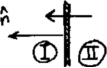
\includegraphics[width=0.3\textwidth]{images/fig_ft1_potencialsketch.pdf}
	\end{center}
	\caption{}
\end{figure} 
\[
	E_I^{\hat{n}} - E_{II}^{\hat{n}} = 4 \pi \sigma \qquad\qquad 
	- \dpar{\phi_I}{x} + \dpar{\phi_{II}}{x} = 4 \pi \sigma
\]

Para $k_{\hat{e}_1}^2$ en el caso discreto
\[
	\sum_{m=0}^\infty \cos(k_m e_1) + \sin(k_m e_1)
\]
pero en el continuo 
\[
	\int_{\infty}^{\infty} \euler^{ike_1} dk
\]
usamos $exp(ike_1)$ para que la integral converja en lugar de $(\cos(ke_1) + \sin(ke_1))$.

% =================================================================================================
\section{Expansiones ortonormales}
% =================================================================================================

\[
	\int_a^b U^*_n U_m d\xi = \delta_{mn} \qquad U_i \; mathrm{ortonormales}
\]
entonces en $(a,b)$ se da que la serie 
\[
	f(\xi) = \sum_{n=0}^\infty a_n U_n(\xi) 
\]
converge, donde  
\[
	a_n = \int_a^b U^*_n f(\xi) d\xi.
\]
La clausura es
\[
	\sum_{n=1}^\infty U^*_n(\vb{x}') U_n(\vb{x}) = \delta(\vb{x}-\vb{x}')
\]

\begin{figure}[thb]
	\begin{center}
	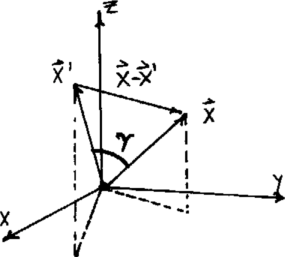
\includegraphics[width=0.4\textwidth]{images/fig_ft1_expansiones1.pdf}	 
	\end{center}
	\caption{}
\end{figure} 

Es útil el desarrollo
\[
	\frac{1}{|\vb{r} - \vb{r}'|} = \frac{1}{\sqrt{r^2 + r'^2 -2rr'\cos(\gamma)}}
	= \sum_{\ell=0}^\infty \frac{r^\ell_{<}}{r^\ell_{>}} P_\ell (\cos(\gamma))
\]
en polinomios de Legendre para el ángulo entre vectores en coordenadas esféricas.
En coordenadas esféricas, donde $\gamma=\gamma(\theta,\phi)$ es el ángulo entre vectores,
que surge del teorema del coseno.

\subsection{Prolongación analítica}

Consiste en {\it prolongar} una solución restringida por ejemplo en el eje polar a todo el
resto del espacio pegándole los polinomios de Legendre.
Lo ponemos en serie (pasamos un cálculo de F3 a una serie)
\[
	\phi(r,\phi/2) = \frac{Q}{\sqrt{r^2 + a^2}} = \sum_{\ell=0}^\infty Q \frac{a^\ell}{r^{\ell + 1}} 
	P_\ell (0) \qquad r > a
\]
\[
	\phi(r,\phi/2) = \frac{Q}{\sqrt{r^2 + a^2}} = \sum_{\ell=0}^\infty Q \frac{r^\ell}{a^{\ell + 1}} 
	P_\ell (0) \qquad r < a
\]
y $P_\ell(0)$ tiene términos pares solamente (los impares son nulos).

\begin{figure}[htb]
	\begin{center}
	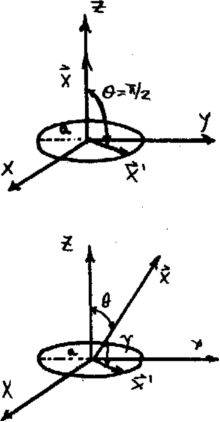
\includegraphics[width=0.3\textwidth]{images/fig_ft1_expansiones2.pdf}	 
	\end{center}
	\caption{}
\end{figure} 

Entonces
\[
	\phi(r,\phi/2) = \frac{Q}{a} \sum_{n=0}^\infty \frac{r^{2n}}{a^{2n}} P_{2n} (0) 
\]
con 
\[
	P_{2n} (0) = (-1)^n \frac{(2n-1)!}{2^n n!}
\]
por lo tanto para todo el espacio será

\begin{figure}[htb]
	\begin{center}
	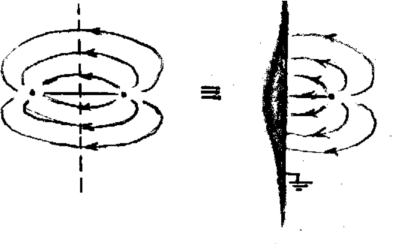
\includegraphics[width=0.4\textwidth]{images/fig_ft1_expansiones3.pdf}	 
	\end{center}
	\caption{}
\end{figure} 

\[
	\phi(r,\phi/2) = \frac{Q}{a} \sum_{n=0}^\infty \left( \frac{r}{a}\right)^{2n} P_{2n} (0) P_{2n} 
	(\sin(\theta)) \qquad r < a
\]
El hecho de que sólo vivan $\ell$ pares viene porque $\phi$ es par pues hay simetría de reflexión en el
plano $xy$, lo que sucede de $(0,\pi/2)$ es igual a lo que sucede de $(\pi/2, \pi)$.

Los problemas con simetría de revolución en torno a $\hat{z}$ pueden ser resueltos con el método de
prolongación analítica. La idea central es que si dos soluciones del potencial coinciden en un conjunto
de puntos (como ser el eje azimutal) entonces deben ser la misma solución.

\subsection{Comentario multipolos}

Estos dos problemas son equivalentes, pero multipolarmente tienen desarrollos diferentes.
El problema es que el metal a tierra tendrá carga hasta el infinito y entonces no podemos tener un
radio de convergencia.


% =================================================================================================
\section{Armónicos esféricos}
% =================================================================================================

\[
	Y_{\ell,m}(\theta,\varphi) = \sqrt{ \frac{ 2\ell + 1}{4\pi} \frac{(\ell-m)! }{(\ell+ m)! } }
	P_\ell^m(\cos(\theta)) \euler^{i m \varphi}
\]
Los armónicos esféricos son un conjunto ortonormalizado en 
\[
	- 1 \leq \cos(\theta) \leq 1 , \qquad 0 \leq \varphi \leq 2\pi
\]
\[
	Y_{\ell,-m}(\theta,\varphi) = (-1) Y_{\ell,m}^*(\theta,\varphi)
\]

La ortonormalidad
\[
	\int_0^{2\pi} d\varphi \int_0^\pi \sin(\theta) Y_{\ell,m}(\theta,\varphi) Y_{\ell,m}^*(\theta,\varphi) d\theta 
	= \delta_{\ell'\ell}\delta_{m'm}
\]
La completitud
\[
	\sum_{\ell=0}^\infty \sum_{m=-\ell}^\ell Y_{\ell,m}(\theta,\varphi) Y_{\ell,m}^*(\theta,\varphi) = 
\delta(\varphi 	-\varphi') \delta(\cos(\theta)-\cos(\theta'))
\]
Entonces una función $f$ cualquiera $\in L^2$ se puede expresar en armónicos esféricos,
\[
	f(\theta,\varphi) = \sum_{\ell=0}^\infty \sum_{m=-\ell}^\ell A_{\ell,m} Y_{\ell,m}(\theta,\varphi)
\]
de manera que el potencial en coordenadas esféricas es
\[
	\phi(r,\theta,\varphi) = \sum_{\ell=0}^\infty \sum_{m=-\ell}^\ell [A_{\ell,m}r^\ell + B_{\ell,m} r^{-(\ell+1)}] 
	Y_{\ell,m}(\theta,\varphi)
\]

Con respecto a la Figura, 

\begin{figure}[bht]
	\begin{center}
	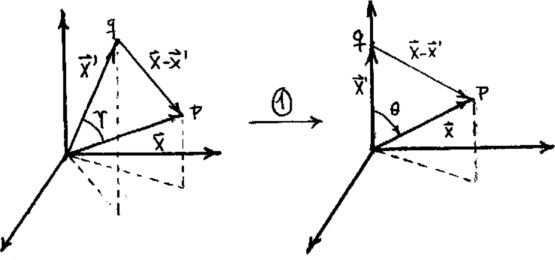
\includegraphics[width=0.7\textwidth]{images/fig_ft1_armesf1.pdf}	 
	\end{center}
	\caption{}
\end{figure} 

si $q$ está en $\hat{z}$ entonces simetría de revolución ($\gamma \to \theta$). Si por el contrario ,
$\gamma $ es nulo entonces simetría de revolución.

\begin{figure}[tb]
	\begin{center}
	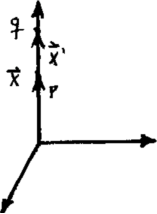
\includegraphics[width=0.3\textwidth]{images/fig_ft1_armesf2.pdf}	 
	\end{center}
	\caption{}
\end{figure} 

Un poco de álgebra de coordenadas,
\[
	\frac{1}{|\vb{x}-\vb{x}'|} = \frac{1}{\sqrt{r^2 + {r'}^2  - 2rr'\cos(\gamma)}} \Rightarrow
	\frac{1}{\sqrt{r^2 + {r'}^2  - 2rr'\cos(\theta)}}
\]
donde $|\vb{x}|=r$ y $|\vb{x}'|=r'$. Así
\[
	\left. \frac{1}{|\vb{x}-\vb{x}'|} \right|_{\gamma=0} = \frac{1}{\sqrt{r^2 + r'^2 -2rr'}}=
	\frac{1}{|r-r'|}
\]
luego si $r'<r$ será
\[
	\frac{1}{|r-r'|} = \frac{1}{r(1 - r'/r )} = \frac{1}{r} \sum_{\ell=0}^\infty \left(\frac{r'}{r}\right)^\ell = 
	\sum_{\ell=0}^\infty \frac{r'^\ell}{r^{\ell+1}}
\]
en cambio si es $r'>r$
\[
	\frac{1}{|r-r'|} = \frac{1}{r'(1 - r/r' )} = \frac{1}{r'} \sum_{\ell=0}^\infty \left(\frac{r}{r'}\right)^\ell = 
	\sum_{\ell=0}^\infty \frac{r^\ell}{r'^{\ell+1}}
\]
de manera que
\[
	\left. \frac{1}{|\vb{x}-\vb{x}'|} \right|_{\gamma=0} = \sum_{\ell=0}^\infty  \frac{r_<^\ell}{r_>^{\ell+1}}
\]
y podemos pensar en $1=P_\ell(1) \forall \ell$ y $1=P_\ell(\cos 0)$
\[
	\left. \frac{1}{|\vb{x}-\vb{x}'|} \right|_{\gamma=0} = \sum_{\ell=0}^\infty  \frac{r_<^\ell}{r_>^{\ell+1}}
	P_\ell(\cos 0)
\]
que será el $\phi$ de una carga unitaria en $\hat{z}$ y evaluado en $\hat{z}$.
Hacemos de esta manera prolongación analítica,
\[
	\frac{1}{|\vb{x}-\vb{x}'|}  = \sum_{\ell=0}^\infty  \frac{r_<^\ell}{r_>^{\ell+1}}
	P_\ell(\cos \gamma)
\]
y decimos que será el $\phi$ de una carga unitaria en cualquier parte (descompuesto en polinomios de Legendre).
Aquí $\gamma=\gamma(\theta,\varphi)$ y se puede llegar a una descomposición similar utilizando armónicos esféricos.

El potencial $\phi$ descompuesto en armónicos esféricos es
\[
	\frac{1}{|\vb{x}-\vb{x}'|}  = \sum_{\ell=0}^\infty \sum_{m=-\ell}^\ell \frac{r_<^\ell}{r_>^{\ell+1}}
	\frac{4\pi}{2\ell+1} Y_{\ell,m}(\theta,\varphi) Y_{\ell,m}^*(\theta',\varphi')
\]
y el teorema de adición de los armónicos esféricos ha sido usado
\[
	P_\ell(\cos \gamma) = \sum_{m=-\ell}^\ell \frac{4\pi}{2\ell+1} Y_{\ell,m}(\theta,\varphi) 
	Y_{\ell,m}^*(\theta',\varphi')
\]

\[
	\phi(\vb{x})= \int_{V'} \rho(\vb{x}')\left[ \sum_{\ell=0}^\infty \sum_{m=-\ell}^\ell 
	\frac{r_<^\ell}{r_>^{\ell+1}}\frac{4\pi}{2\ell+1} Y_{\ell,m}(\theta,\varphi) 
	Y_{\ell,m}^*(\theta',\varphi')\right] dV',
\]
que se puede cosmetizar como
\[
	\phi(\vb{x})= 4\pi \sum_{\ell=0}^\infty \sum_{m=-\ell}^\ell \frac{1}{2\ell+1} \left[
	\int_{V'} \rho(\vb{x}') Y_{\ell,m}^*(\theta',\varphi') {r'}_<^\ell dV' \right] 
	\frac{Y_{\ell,m}(\theta,\varphi) }{r_>^{\ell+1}},
\]
definiéndose el corchete como $q_{\ell m}$ coeficiente multipolar de orden $\ell m$, así
\[
	\phi(\vb{x})= 4\pi \sum_{\ell=0}^\infty \sum_{m=-\ell}^\ell \frac{q_{\ell m}}{2\ell+1} 
	\frac{Y_{\ell,m}(\theta,\varphi) }{r_>^{\ell+1}}.
\]

Entonces
\[
	\phi_{\ell m}(\vb{x})= 4\pi \frac{q_{\ell m}}{2\ell+1}\frac{Y_{\ell,m}(\theta,\varphi) }{r_>^{\ell+1}}
\]
y consecuentemente
\[
	\vb{E}_{\ell m}(\vb{x}) = - \Nabla \phi_{\ell m}(\vb{x})
\]

% =================================================================================================
\section{Separación de variables en cilíndricas}
% =================================================================================================

Se propone
\[
	\phi(\rho,\phi,z) = R(\rho) Q(\phi) Z(z)
\]
de modo que
\[
	\frac{1}{R} \dtot[2]{R}{\rho} + \frac{1}{R\rho} \dtot{R}{\rho} + \frac{1}{Q\rho^2} \dtot[2]{Q}{\phi} 
				+ \frac{1}{Z} \dtot[2]{Z}{z} = 0
\]
donde los primeros dos términos conducen a la ecuación de Bessel, el tercero es igual a $-\nu^2$ y el
cuarto a $k^2$. Sacamos
\[
	Z = \euler^{\pm kz}
\]
\[
	Q = \euler^{\pm i \nu \phi}
\]
donde si $0\leq \phi \leq 2\pi$ entonces $\nu \in \mathbb{Z}$. Si en cambio la variable $\phi$ no corre 
entre $0$ a $2\pi$ se dará que $\nu \notin \mathbb{Z}$.

\begin{center}
	\begin{tabular}{|c|c|}
	\hline
	$ \nu \in \mathbb{Z} $ & $ \nu \notin \mathbb{Z}  $ \\
	\hline
	$J_\nu(k\rho)$ & $J_\nu(k\rho)$ \\
	$J_{-\nu}(k\rho)$ & $N_\nu(k\rho)$ \\
	\hline
	\end{tabular} 
\end{center}
donde 
\[
	N_\nu(k\rho) \equiv \frac{ J_\nu(k\rho) \cos(\nu\pi) - J_{-\nu}(k\rho)}{\sin(\nu\pi)}
\]
siendo $J_\nu(k\rho)$ la función de Bessel de primera especie, $N_\nu(k\rho)$ la función de Bessel de segunda 
especie (Neumann).
$N_\nu(k\rho)$ tiene problemas en el origen de modo que no sirve si el dominio incluye al eje $\hat{z}$, en 
cambio $J_\nu(k\rho)$ tiene problemas en $\rho\to \infty$.

También se suelen definir
\[
	H^{(1)}_\nu(k\rho) = J_\nu(k\rho) + i N_\nu(k\rho)
\]
\[
	H^{(2)}_\nu(k\rho) = J_\nu(k\rho) - i N_\nu(k\rho)
\]
que son las funciones de Bessel de tercera especie o bien Hankel de primera y segunda especie respectivamente.

\subsubsection{Cambio de signo de la constante de separación}

\[
	... + \underbrace{\frac{1}{Z} \dtot[2]{Z}{z}}_{-k^2} =  0
\]
entonces nos lleva a
\[
	Z = \euler^{\pm i k z} \qquad \qquad Q = \euler^{\pm i \nu \phi}
\]
y entonces a las funciones de Bessel modificadas
\[
	I_\nu(k\rho) = i^{-\nu} J_\nu(k\rho)
\]
\[
	K_\nu(k\rho) = \frac{\pi}{2}i^{\nu+1} H_\nu^{(1)}(k\rho),
\]
donde son respectivamente las de primera y segunda especie y vemos que tienen argumento imaginario.
Las $I_\nu(k\rho)$ tendrán problemas en $\rho\to\infty$ y $K_\nu(k\rho)$ problemas en $\rho=0$ (en el eje 
$\hat{z}$).
Si atravesamos densidades de carga en $\hat{z}$ entonces usamos Bessel
\[
	Z = \euler^{\pm k z} \quad \Rightarrow \quad J_\nu^{(1)}(k\rho) ; N_\nu^{(2)}(k\rho)
\]
pero bajo condiciones periódicas en $\hat{z}$ se usan Bessel modificadas
\[
	Z = \euler^{ \pm i k z} \quad \Rightarrow \quad I_\nu^{(1)}(k\rho) ; K_\nu^{(2)}(k\rho)
\]
y esto último se da por ejemplo en tapas del cilindro.
La función de Bessel de primera especie se puede expresar como serie según
\[
	J_\nu^{(1)}(k\rho) = \left(\frac{x}{2}\right)^\nu \sum_{j=0}^\infty \frac{(-1)^j}{j!\Gamma(j+\nu +1)} 
		\left(\frac{x}{2}\right)^{2j}
\]

Las funciones de Bessel tienen infinitos ceros,
\[
	J_\nu(x_{\nu n}) = 0 \qquad \mathrm{con} \; n\in\mathbb{N}, \nu \quad \mathrm{fijo} 
\]
siendo $x_{\nu n}$ un cero de $J_\nu$. Así
\[
	\sqrt{\rho} J_\nu(x_{\nu n} \rho/a) 
\]
con $\nu \geq 0$ fijo es un conjunto ortonormal completo en $0 \leq \rho \leq a$ siendo $a$ el radio del 
cilindro.
\[
	f(\rho) = \sum_{n=1}^{\infty}  A_{x_{\nu n}} J_{\nu}( x_{\nu n} \rho/a )
\]
con $0 \leq \rho \leq a$. Así $f(\rho=a)=0$,
\[
	A_{\nu n} = \frac{2}{a^2 J_{\nu +1}^2 (x_{\nu n})} \int_0^a \rho f(\rho) J_\nu (x_{\nu n} \rho/a) 
	d\rho
\]
la ortogonalidad
\[
	\int_0^a \rho  J_\nu (x_{\nu n'} \rho/a)  J_\nu (x_{\nu n} \rho/a)  d\rho = 
	\frac{a^2}{2}[J_{\nu+1}(x_{\nu n})]^2 \delta_{nn'}.
\]

Para $k$ sea $\phi(\rho=a)=0$ entonces 
\[
	J_\nu(ka) = 0 \Rightarrow ka=x_{\nu n} \Rightarrow J_\nu (x_{\nu n} \rho/a)
\]
y $k=\frac{x_{\nu n}}{a}$ si $0\leq \rho \leq a$ y si está acotado en $\rho$ entonces es discreto y se
suma $\sum_{n=1}^\infty$ y $\nu\to m \in \mathbb{Z}$ si $0 \leq \phi \leq 2\pi$ y si no está acotado en
$\rho$ entonces usamos 
\[
	\int_0^\infty dk
\]
y la completitud
\[
	\int_0^\infty x J_\nu(kx) J_\nu(k'x) dx = \frac{1}{k} \delta (k-k')
\]
y $k$ en general será función de $n\in \mathbb{N}$ por condición periódica en tapas (en $\hat{z}$) o en
cilindros (en $\hat{\rho}$).
\[
	\phi(\rho,\phi,z) = \sum_{\nu=0}^\infty \sum_{n=1}^\infty
	[A_{\nu k}\begin{cases} J_\nu(k\rho)  \\ I_\nu(k\rho) \end{cases} + 
	B_{\nu k} \begin{cases} N_\nu(k\rho)  \\ K_\nu(k\rho) \end{cases} ]
	[C_k \begin{cases} \euler^{\pm kz} \\ \euler^{\pm ikz} \end{cases}]
	[D_{k\nu} \euler^{\pm i \nu \phi}]
\]
donde $k=k(n)$ y usamos $\sin(kz)+\cos(kz)$ si hay discretización.



% \bibliographystyle{CBFT-apa-good}	% (uses file "apa-good.bst")
% \bibliography{CBFT.Referencias} % La base de datos bibliográfica

\end{document}

	
		\documentclass[10pt,oneside]{CBFT_book}
	% Algunos paquetes
	\usepackage{amssymb}
	\usepackage{amsmath}
	\usepackage{graphicx}
	\usepackage{libertine}
	\usepackage[bold-style=TeX]{unicode-math}
	\usepackage{lipsum}

	\usepackage{natbib}
	\setcitestyle{square}

	\usepackage{polyglossia}
	\setdefaultlanguage{spanish}


	\usepackage{CBFT.estilo} % Cargo la hoja de estilo

	% Tipografías
	% \setromanfont[Mapping=tex-text]{Linux Libertine O}
	% \setsansfont[Mapping=tex-text]{DejaVu Sans}
	% \setmonofont[Mapping=tex-text]{DejaVu Sans Mono}

	%===================================================================
	%	DOCUMENTO PROPIAMENTE DICHO
	%===================================================================

\begin{document}

% =================================================================================================
\chapter{Expansión en un campo multipolar}
% =================================================================================================

% =================================================================================================
\section{Desarrollo dipolar del campo magnético}
% =================================================================================================

El potencial vector de un dipolo es
\[
	\vb{A}(\vb{x}) = \frac{\vb{v}\times(\vb{x}-\vb{x}')}{|\vb{x}-\vb{x}'|^3} = \vb{m} \times \Nabla 
		\frac{1}{|\vb{x}-\vb{x}'|}
\]
\[
	\vb{A}(\vb{x}) = \int_{V'} \vb{\mathcal{M}}(\vb{x}') \times \Nabla 
			\left(\frac{1}{|\vb{x}-\vb{x}'|}\right) dV'
\]
Es el potencial vector de una distribución de momento dipolar magnético con densidad $ \vb{M}(\vb{x}')$

\[
	\vb{A}(\vb{x}) = \int_{V'} \frac{\rotorm{\vb{M}}}{|\vb{x}-\vb{x}'|} dV' +
			\int_{S'} \frac{\vb{M}\times\hat{n}}{|\vb{x}-\vb{x}'|} dS'
\]
y se pueden pensar como corrientes $\vb{J}_M$ y $\vb{g}_M$,
\[
	\vb{A}(\vb{x}) = \frac{1}{c} \int_{V'} \frac{\vb{J}_M}{|\vb{x}-\vb{x}'|} dV' +
			\frac{1}{c} \int_{S'} \frac{\vb{g}_M}{|\vb{x}-\vb{x}'|} dS'
\]

% =================================================================================================
\section{Medios materiales}
% =================================================================================================

\begin{itemize}
 \item Dieléctricos
 \item Medios magnéticos
	$\begin{cases}
	 \text{imán inducido} \\
	 \text{imán permanente}
	\end{cases}$
 \item Conductor
	$\begin{cases}
	 \text{perfecto} \\
	 \text{buen conductor} \\
	 \text{mal conductor}
	\end{cases}$
\end{itemize}


% =================================================================================================
\section{Desarrollo multipolar}
% =================================================================================================






% =================================================================================================
\section{Dipolo}
% =================================================================================================









% =================================================================================================
\section{Campo dipolar}
% =================================================================================================













% \bibliographystyle{CBFT-apa-good}	% (uses file "apa-good.bst")
% \bibliography{CBFT.Referencias} % La base de datos bibliográfica

\end{document}

	
		\documentclass[10pt,oneside]{CBFT_book}
	% Algunos paquetes
	\usepackage{amssymb}
	\usepackage{amsmath}
	\usepackage{graphicx}
	\usepackage{libertine}
	\usepackage[bold-style=TeX]{unicode-math}
	\usepackage{lipsum}

	\usepackage{natbib}
	\setcitestyle{square}

	\usepackage{polyglossia}
	\setdefaultlanguage{spanish}


	\usepackage{CBFT.estilo} % Cargo la hoja de estilo

	% Tipografías
	% \setromanfont[Mapping=tex-text]{Linux Libertine O}
	% \setsansfont[Mapping=tex-text]{DejaVu Sans}
	% \setmonofont[Mapping=tex-text]{DejaVu Sans Mono}

	%===================================================================
	%	DOCUMENTO PROPIAMENTE DICHO
	%===================================================================

\begin{document}

% =================================================================================================
\chapter{ }
% =================================================================================================





% \bibliographystyle{CBFT-apa-good}	% (uses file "apa-good.bst")
% \bibliography{CBFT.Referencias} % La base de datos bibliográfica

\end{document}

	
		\documentclass[10pt,oneside]{CBFT_book}
	% Algunos paquetes
	\usepackage{amssymb}
	\usepackage{amsmath}
	\usepackage{graphicx}
	\usepackage{libertine}
	\usepackage[bold-style=TeX]{unicode-math}
	\usepackage{lipsum}

	\usepackage{natbib}
	\setcitestyle{square}

	\usepackage{polyglossia}
	\setdefaultlanguage{spanish}


	\usepackage{CBFT.estilo} % Cargo la hoja de estilo

	% Tipografías
	% \setromanfont[Mapping=tex-text]{Linux Libertine O}
	% \setsansfont[Mapping=tex-text]{DejaVu Sans}
	% \setmonofont[Mapping=tex-text]{DejaVu Sans Mono}

	%===================================================================
	%	DOCUMENTO PROPIAMENTE DICHO
	%===================================================================

\begin{document}

% =================================================================================================
\chapter{Ondas planas}
% =================================================================================================



% =================================================================================================
\section{Polarización de ondas}
% =================================================================================================

\begin{figure}[htb]
	\begin{center}
	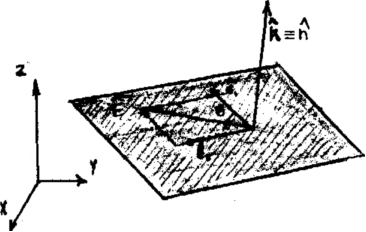
\includegraphics[width=0.4\textwidth]{images/fig_ft1_polariz.pdf}	 
	\end{center}
	\caption{}
\end{figure} 

% =================================================================================================
\section{Reflexión y refracción de ondas en medios}
% =================================================================================================

\begin{figure}[htb]
	\begin{center}
	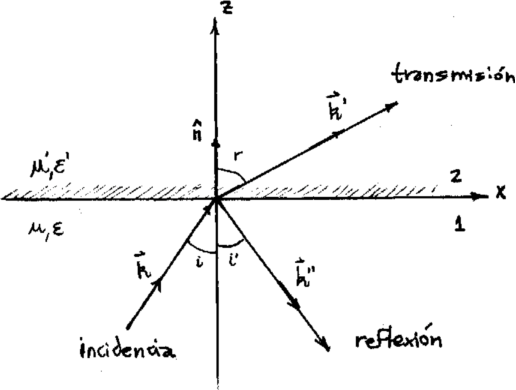
\includegraphics[width=0.4\textwidth]{images/fig_ft1_reflex1.pdf}	 
	\end{center}
	\caption{}
\end{figure} 

\begin{figure}[htb]
	\begin{center}
	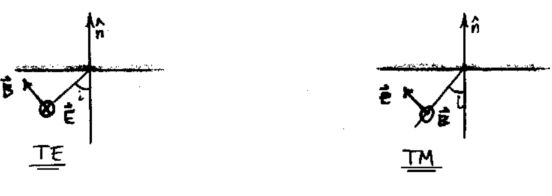
\includegraphics[width=0.4\textwidth]{images/fig_ft1_reflex2.pdf}	 
	\end{center}
	\caption{}
\end{figure} 

\begin{figure}[htb]
	\begin{center}
	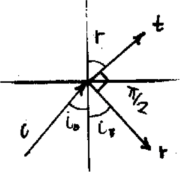
\includegraphics[width=0.4\textwidth]{images/fig_ft1_reflex3.pdf}	 
	\end{center}
	\caption{}
\end{figure} 

\begin{figure}[htb]
	\begin{center}
	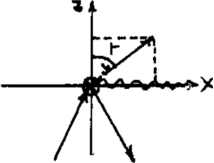
\includegraphics[width=0.4\textwidth]{images/fig_ft1_reflex4.pdf}	 
	\end{center}
	\caption{}
\end{figure} 

% =================================================================================================
\section{Campo electromagnético en un medio conductor}
% =================================================================================================

\begin{figure}[htb]
	\begin{center}
	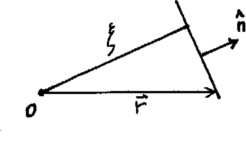
\includegraphics[width=0.4\textwidth]{images/fig_ft1_conduc1.pdf}	 
	\end{center}
	\caption{}
\end{figure} 

\begin{figure}[htb]
	\begin{center}
	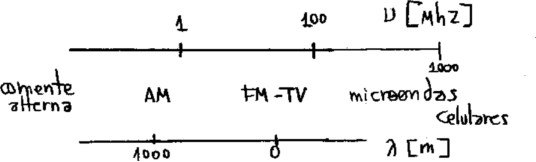
\includegraphics[width=0.4\textwidth]{images/fig_ft1_conduc2.pdf}	 
	\end{center}
	\caption{}
\end{figure} 

\begin{figure}[htb]
	\begin{center}
	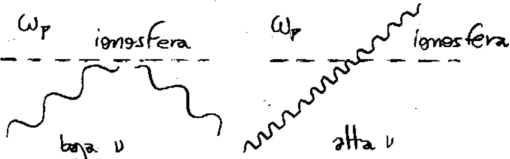
\includegraphics[width=0.4\textwidth]{images/fig_ft1_conduc3.pdf}	 
	\end{center}
	\caption{}
\end{figure} 

\begin{figure}[htb]
	\begin{center}
	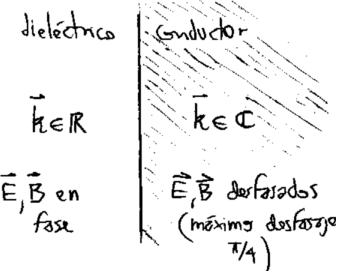
\includegraphics[width=0.4\textwidth]{images/fig_ft1_conduc4.pdf}	 
	\end{center}
	\caption{}
\end{figure} 

% =================================================================================================
\section{Transformación de vectores}
% =================================================================================================

\begin{figure}[htb]
	\begin{center}
	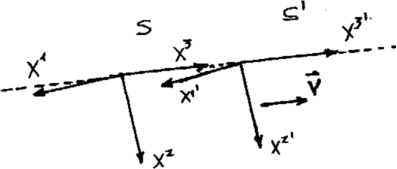
\includegraphics[width=0.4\textwidth]{images/fig_ft1_transfvec.pdf}	 
	\end{center}
	\caption{}
\end{figure} 


\subsection{Intervalos}

\begin{figure}[htb]
	\begin{center}
	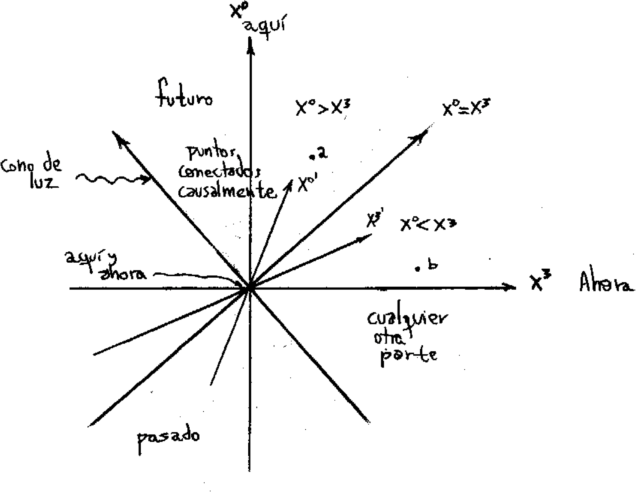
\includegraphics[width=0.4\textwidth]{images/fig_ft1_intervalos.pdf}	 
	\end{center}
	\caption{}
\end{figure} 

\subsection{Transcurso del tiempo en un sistema con V grande}

\begin{figure}[htb]
	\begin{center}
	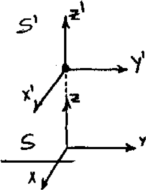
\includegraphics[width=0.4\textwidth]{images/fig_ft1_vgrande.pdf}	 
	\end{center}
	\caption{}
\end{figure} 




% \bibliographystyle{CBFT-apa-good}	% (uses file "apa-good.bst")
% \bibliography{CBFT.Referencias} % La base de datos bibliográfica

\end{document}

	
		\documentclass[10pt,oneside]{CBFT_book}
	% Algunos paquetes
	\usepackage{amssymb}
	\usepackage{amsmath}
	\usepackage{graphicx}
	\usepackage{libertine}
	\usepackage[bold-style=TeX]{unicode-math}
	\usepackage{lipsum}

	\usepackage{natbib}
	\setcitestyle{square}

	\usepackage{polyglossia}
	\setdefaultlanguage{spanish}


	\usepackage{CBFT.estilo} % Cargo la hoja de estilo

	% Tipografías
	% \setromanfont[Mapping=tex-text]{Linux Libertine O}
	% \setsansfont[Mapping=tex-text]{DejaVu Sans}
	% \setmonofont[Mapping=tex-text]{DejaVu Sans Mono}

	%===================================================================
	%	DOCUMENTO PROPIAMENTE DICHO
	%===================================================================

\begin{document}

% =================================================================================================
\chapter{Relatividad especial}
% =================================================================================================


% =================================================================================================
\section{Transformación de los campos}
% =================================================================================================

\begin{figure}[htb]
	\begin{center}
	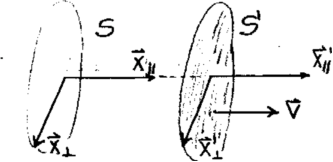
\includegraphics[width=0.4\textwidth]{images/fig_ft1_transfCampo1.pdf}	 
	\end{center}
	\caption{}
\end{figure} 

\begin{figure}[htb]
	\begin{center}
	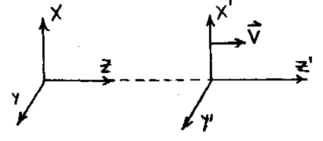
\includegraphics[width=0.4\textwidth]{images/fig_ft1_transfCampo2.pdf}	 
	\end{center}
	\caption{}
\end{figure} 



% =================================================================================================
\section{Especie de tiro oblicuo}
% =================================================================================================

\begin{figure}[htb]
	\begin{center}
	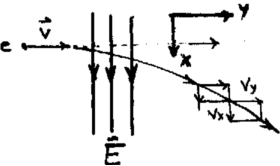
\includegraphics[width=0.4\textwidth]{images/fig_ft1_tirooblicuo.pdf}	 
	\end{center}
	\caption{}
\end{figure} 

% =================================================================================================
\section{cuadrivelocidad}
% =================================================================================================


\begin{figure}[htb]
	\begin{center}
	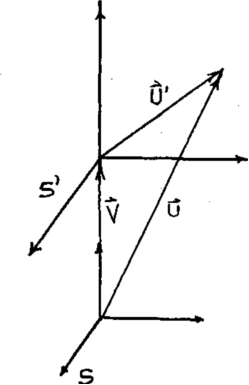
\includegraphics[width=0.4\textwidth]{images/fig_ft1_4vel.pdf}	 
	\end{center}
	\caption{}
\end{figure} 

% \bibliographystyle{CBFT-apa-good}	% (uses file "apa-good.bst")
% \bibliography{CBFT.Referencias} % La base de datos bibliográfica

\end{document}

	
		\documentclass[10pt,oneside]{CBFT_book}
	% Algunos paquetes
	\usepackage{amssymb}
	\usepackage{amsmath}
	\usepackage{graphicx}
	\usepackage{libertine}
	\usepackage[bold-style=TeX]{unicode-math}
	\usepackage{lipsum}

	\usepackage{natbib}
	\setcitestyle{square}

	\usepackage{polyglossia}
	\setdefaultlanguage{spanish}


	\usepackage{CBFT.estilo} % Cargo la hoja de estilo

	% Tipografías
	% \setromanfont[Mapping=tex-text]{Linux Libertine O}
	% \setsansfont[Mapping=tex-text]{DejaVu Sans}
	% \setmonofont[Mapping=tex-text]{DejaVu Sans Mono}

	%===================================================================
	%	DOCUMENTO PROPIAMENTE DICHO
	%===================================================================

\begin{document}

% =================================================================================================
\chapter{Campos de cargas en movimiento}
% =================================================================================================

% =================================================================================================
\section{Potenciales retardados}
% =================================================================================================

Usando el gauge de Lorentz y las ecuaciones de Maxwell se llega a
\[
	\lapm{\vb{A}} - \frac{1}{c^2} \dpar[2]{\vb{A}}{t} = -\frac{4\pi}{c} \vb{J}
\]
\[
	\lapm{\phi} - \frac{1}{c^2} \dpar[2]{\phi}{t} = - 4 \pi \phi
\]
con forma general 
\be
	\lapm{\psi} - \frac{1}{c^2} \dpar[2]{\psi}{t} = - 4 \pi f(\vb{x},t)
	\label{onda_general}
\ee
siendo $f$ la que da la distribución de fuentes.

Resolveremos \eqref{onda_general} con una función de Green. Hacemos Fourier respecto a la frecuencia, de
manera que podamos remover el tiempo (además luego nos interesarán fuentes armónicas y por sobre todo
cualquier perturbación puede descomponerse en Fourier).

Suponemos que podemos escribir
\[
	\psi(\vb{x},t) = \frac{1}{2\pi}\int_{-\infty}^{+\infty} \psi(\vb{x},\omega) \euler^{-i\omega t} 
	d\omega
\]
\[
	f(\vb{x},t) = \frac{1}{2\pi}\int_{-\infty}^{+\infty} f(\vb{x},\omega) \euler^{-i\omega t} d\omega
\]
siendo sus inversas
\[
	\psi(\vb{x},\omega) = \int_{-\infty}^{+\infty} \psi(\vb{x}, t) \euler^{i\omega t} dt
\]
\[
	f(\vb{x},\omega) = \int_{-\infty}^{+\infty} f(\vb{x},t) \euler^{i\omega t} dt
\]
luego la ecuación resulta 
\[
	\int_{-\infty}^{+\infty} \lapm{\psi}(\vb{x},\omega) \euler^{ -i\omega t} d\omega +
	\int_{-\infty}^{+\infty} \frac{\omega^2}{c^2}\psi(\vb{x},\omega) \euler^{ -i\omega t} d\omega = 
		- 4 \pi \int_{-\infty}^{+\infty} f(\vb{x},\omega) \euler^{ -i\omega t} d\omega
\]
de manera que se satisface la ecuación de Helmholtz inhomogénea,
\[
	(\nabla^2 + k^2)\psi(\vb{x},\omega) = - 4\pi f(\vb{x},\omega),
\]
para cada valor de frecuencia $\omega$.

Una función de Green satisfacerá 
\[
	(\nabla^2 + k^2) G(\vb{x},\vb{x}') = - 4\pi \delta(\vb{x}-\vb{x}'),
\]
donde $\vb{x}-\vb{x}' = \vb{R}$ y la función de Green será simétricamente esférica pues pedimos la
no existencia de contornos, entonces llamando a aquella $G_k(R)$ se tiene 
\[
	\frac{1}{R}\dtot[2]{}{R}(RG_k) + k^2 G_k = - 4 \pi \delta (\vb{R})
\]
donde hemos usado el laplaciano en esféricas. Debemos distinguir dos casos, si $R=0$ entonces la
anterior resulta 
\[
	\lim_{kR \to 0} G_k(R) = \frac{1}{R}
\]
mientras que de ser cierto $R\neq 0$ en cambio
\[
	\dtot[2]{}{R}(RG_k) + k^2 (RG_k) = 0
\]
y entonces se propone como solución general 
\[
	G_k(R) = \frac{ A }{ R } \euler^{ i k R } + \frac{ B }{ R } \euler^{ -i k R }
\]
donde $A, B$ dependerán de las condiciones de contorno y siendo que el primer término del RHS representa
una onda divergente esférica y el segundo una onda convergente esférica.

Se puede interpretar $G_k$ como el potencial de una carga unitaria que aparece en $\vb{x}=\vb{x}'$ en el
instante $t=t'$ y luego desaparece (mmm, qué misterio!).

Ahora necesitamos meter la dependencia temporal,
\[
	\left(\nabla^2_x - \frac{1}{c^2}\dpar[2]{}{t} \right) G^{\pm}(\vb{x},\vb{x}',t,t') = 
	- 4 \pi \delta(\vb{x}-\vb{x}') \delta(t-t')
\]
\[
	- 4 \pi f(\vb{x},\omega) = -4 \pi \int_{-\infty}^{+\infty} f(\vb{x},t) \euler^{i\omega t} dt =
		-4 \pi \int_{-\infty}^{+\infty} \delta(\vb{x}-\vb{x}') \delta(t-t') \euler^{i\omega t} dt
\]
\[
	- 4 \pi f(\vb{x},\omega) = -4 \pi \delta(\vb{x}-\vb{x}') \euler^{i\omega t'} 
\]
de modo que tenemos 
\[
	f(\vb{x},\omega) = \delta(\vb{x}-\vb{x}') \euler^{i\omega t'} ,
\]
usando lo cual se llega a
\[
	G^{\pm}(R,\tau) = \frac{1}{2\pi} \int_{-\infty}^{+\infty} G_k(R) \euler^{-\omega t} d\omega
\]
donde $\tau$ es el tiempo relativo entre los tiempos de observación y fuente ($t'$ ) y $R$ es la distancia 
relativa entre observación y fuente.

En un medio no dispersivo es 
\[
	G^{\pm}(R,\tau) = \frac{1}{R} \delta( \tau \mp \frac{R}{c})
\]
y así llegamos a
\[
	G^+(\vb{x},\vb{x}',t,t') = \frac{1}{|\vb{x} - \vb{x}'|} \delta( t-t' - \frac{1}{c}(\vb{x} - 
	\vb{x}')) = \frac{ \delta(t' - [t-(1/c)|\vb{x} - \vb{x}'|]) }{|\vb{x} - \vb{x}'|} ,
\]
la función de Green retardada
\[
	G^-(\vb{x},\vb{x}',t,t') = \frac{1}{|\vb{x} - \vb{x}'|} \delta( t-t' + \frac{1}{c}(\vb{x} - 
	\vb{x}')) = \frac{ \delta(t' - [t + (1/c)|\vb{x} - \vb{x}'|]) }{|\vb{x} - \vb{x}'|},
\]
la función de Green avanzada.

$G^+$ exhibe el comportamiento causal del efecto observado en \vb{x} a $t$ causado por la acción de la
fuente en el tiempo $(t-R/c)$ donde $R/c$ es la diferencia de tiempo de la señal en propagarse.
Al valor 
\[
	t' = t - \frac{R}{c}
\]
se lo llama el tiempo retardado. Es un poco más práctica la nomenclatura
\[
	G^+(R,t,t') = \frac{ \delta(t' - [ t - (R/c) ]) }{ R } 
	\qquad 
	G^-(R,t,t') = \frac{ \delta(t' - [ t + (R/c) ]) }{ R } ,
\]

Entonces una solución particular de (1) (¿uno qué?) es 
\[
	\psi^\pm (\vb{x},t) = \int \int G^{\pm}(\vb{x},\vb{x}',t,t') f(\vb{x}',t') d^3x' dt' 
\]
y dos soluciones son 
\[
	\psi_{in}(\vb{x},t) + \int\int G^+ f dv' dt \qquad \qquad \psi_{s}(\vb{x},t) + \int\int G^- f dv' dt
\]
con $f(\vb{x}',t')$ una fuente que es diferente de cero solo en un intervalo $\sim t'$. Entonces $\psi_{in}$ 
satisface (1) homogénea en $t \to -\infty$. $\psi_{s}$ es la onda en $t \to +\infty$ solución homogénea.
La situación más común es el caso de $\psi_{in}$ con $\psi_{in}=0$ entonces 
\[
	\psi (\vb{x},t) = \int_{-\infty}^{+\infty} \int_v' \frac{\delta(t'-[t -(R/c) ]) }{ R } 
			f(\vb{x}',t') dv' dt',
\]
e integrando con la delta
\[
	\psi (\vb{x},t) = \int_v' \frac{ f( \vb{x}', t -(R/c) ) }{ R } dv',
\]
que es una fuente en una cierta región que se enciende un instante e irradia.

\subsection{Fuente armónica}

Sea una fuente armónica en el tiempo 
\[
	\vb{J}(\vb{x}', t') = \vb{J}(\vb{x}') \euler^{-i\omega t'}
\]
entonces el potencial vector es 
\[
	\vb{A}(\vb{x}, t) = \left. \frac{4\pi}{c} \int_v' \frac{\vb{J}(\vb{x}')}{|\vb{x} - \vb{x}'|} 
	\euler^{-i\omega t'} \right|_{t_{ret}} dv' = \left. \frac{4\pi}{c} \int_v' 
	\frac{\vb{J}(\vb{x}')}{|\vb{x} - \vb{x}'|} \euler^{-i \omega t} \euler^{i \omega R/c } 
	\right|_{t_{ret}} dv'
\]
\[
	\vb{A}(\vb{x}, t) = \frac{4\pi}{c} \euler^{-i \omega t} \int_v \frac{\vb{J}(\vb{x})}{ R }
		\euler^{i \omega R/c } dv
\]
se puede ver como 
\[
	\vb{A}(\vb{x}) \euler^{-i \omega t} = \frac{4\pi}{c} \int_v' \frac{\vb{J}(\vb{x}')}{|\vb{x}-\vb{x}'|}
		\euler^{i k |\vb{x}-\vb{x}'| } dv' \euler^{-i \omega t}
\]

Si la fuente oscila armónicamente con frecuencia $\omega$ entonces los campos tendrán la misma frecuencia 
$\omega$.
\[
	\vb{A}(\vb{x}) = \frac{1}{c} \int_v' \frac{\vb{J}(\vb{x}')}{|\vb{x}-\vb{x}'|}
		\euler^{i \omega/c |\vb{x}-\vb{x}'| } dv'
\]
y 
\[
	\vb{A}(\vb{x},t) = \vb{A}(\vb{x}) \euler^{-i \omega t} \quad \text{si} \quad
		\vb{J}(\vb{x}',t') = \vb{J}(\vb{x}') \euler^{-i \omega t'}
\]
La aproximación consiste en desarrollar 
\[
	\frac{\euler^{i k |\vb{x}-\vb{x}'| }}{|\vb{x}-\vb{x}'|}
\]
y ver condiciones asintóticas. Cuando $\ell = 0$ (el primer término de la sumatoria en $\ell$) y
$ kx' \ll 1$ tenemos una antena ineficiente. La longitud de onda $\lambda$ de la radiación es mucho mayor al 
tamaño del emisor, $ 2\pi x' \ll \lambda$ (longitud de onda larga).
En cambio tenemos $ 2\pi x \gg \lambda$ que es la condición de campo lejano (siempre la usaremos).

Por lo tanto,
\[
	\vb{A}(\vb{x})^{(0)} = - i k \vb{p} \frac{\euler^{ikx}}{x}
\]
es una onda esférica saliente. Es el potencial vector \vb{A} de un dipolo magnético oscilante armónicamente.
Recordemos que falta siempre {\it pegarle} un factor $\exp(i\omega t)$. Usando $\vb{E} 0 i/k \rotorm{B}, 
\vb{B} = \rotorm{A}$ tenemos 
\be
	\vb{B}(\vb{x})^{(0)} = k^2 (\hat{r}\times\vb{p})\frac{\euler^{ikx}}{x}\left(1 -\frac{1}{ikx}\right)
	\label{B_rad}
\ee
siendo $\hat{r}$ la dirección de propagación y $x\equiv|\vb{x}|$ que puede ser $|r\hat{r}|$ en esféricas.
El que contribuye a la radiación es el primer término de \eqref{B_rad} (campo lejano) mientras que el segundo
se va a cero rápidamente.

Cerca de la antena es 
\[
	\vb{B}(\vb{x})^{(0)} = i k (\hat{r}\times\vb{p})\frac{1}{r^2}, 
\]
pues $kx\ll 1$ y entonces $\exp(ikx) \sim 1$ (campo cercano) de manera que si $\lambda \to \infty$ entonces
$\vb{B}^{(0)} \sim 0$. El campo \vb{E} cerca de la antena es
\[
	\vb{E} = \frac{i}{k}\rotorm{B} \qquad \rightarrow \quad 
	\vb{E}^{(0)} = \frac{3\hat{r}(\hat{r}\cdot\vb{p}) - \vb{p}}{r^3}
\]
que es el campo de un dipolo eléctrico. $\vb{E},\vb{B}$ son transversales a $\hat{r}$ y tienen la misma 
longitud (en unidades CGS).
La potencia media (en un número entero de períodos) será 
\[
	\langle dP \rangle = \langle\vb{S}\rangle\cdot d\vb{S} = \langle \vb{S}\rangle\cdot\hat{n}r^2 d\Omega
\]
y entonces
\[
	\langle\frac{dP}{d\Omega}\rangle = \langle\vb{S}\rangle\cdot\hat{n}r^2 
\]
\[
	\langle\frac{dP}{d\Omega}\rangle = \frac{c}{8\pi} k^4 p^2 \sin(\theta)^2 
\]
y este cálculo podemos ver de dónde sale 
\[
	\langle\vb{S}\rangle = \frac{c}{2 4 \pi} \re\{ \vb{E}\times\vb{B}^* \} =
		\frac{c}{8\pi} \re\{ ( \vb{B}^0 \times \hat{r} )\times k^2(\hat{r} \times \vb{p})/r \}
\]
\[
	\langle\vb{S}\rangle =
	\frac{c}{8\pi} \re\{(-p k^2/r \sin(\theta) \hat{\theta})\times(-p k^2/r\sin(\theta)\hat{\phi} \}
	= \frac{c}{8\pi} p^2 k^4 \sin(\theta)^2 \hat{r}\cdot\hat{r}
\]
\notamargen{Tenemos un cálculo auxiliar de esta cuenta pero no sé si suma meterlo acá.}

Luego, la potencia irradiada es máxima en $\theta=\pi/2$ (ver figura)

\begin{figure}[htb]
	\begin{center}
	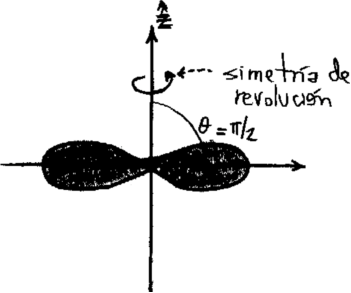
\includegraphics[width=0.4\textwidth]{images/fig_ft1_pot_irrad.pdf}	 
	\end{center}
	\caption{}
\end{figure} 

Entonces, 
\begin{itemize}
 \item Si $\vb{B}=0$ se da que $\vb{S}=0$, es decir que no hay radiación.
 \item Un monopolo no produce campo de radiación por su simetría esférica.
 Una corriente $J\hat{r}$ no produce \vb{B} y se tienen
 \[
	\vb{B}^0_{rad} = \frac{k^2}{r}( \hat{r} \times \vb{p} ) \euler^{ikr} \qquad \qquad 
	\vb{E}^0_{rad} = \frac{k^2}{r}( \hat{r} \times \vb{p} ) \euler^{ikr} \times \hat{r}
 \]
	\begin{figure}[htb]
		\begin{center}
		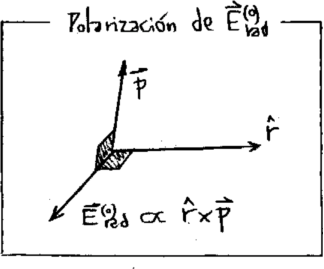
\includegraphics[width=0.4\textwidth]{images/fig_ft1_pot_irrad2.pdf}	 
		\end{center}
		\caption{}
	\end{figure} 
 \item Para que un campo sea de radiación debe tener flujo \vb{S} no nulo en el infinito.
 Si los campos van como $1/r$ entonces el Poynting va como $1/r^2$ y $dS$ va como $r^2$
 de modo que $\langle\vb{S}\rangle \cdot d\vb{S}$ tiene valor constante (un flujo que se
 va y no retorna a la fuente). Si el campo va como $1/r^2$ y entonces no produce flujo
 lejos.
 \item Si hacemos la aproximación $\ell=1$ en $\sum_\ell$ resulta que se obtiene un momento
 magnético oscilante más un cuadrupolo eléctrico.
 \item La radiación a orden $\ell=0$ es un dipolo eléctrico oscilante (ver figura)
	\begin{figure}[htb]
		\begin{center}
		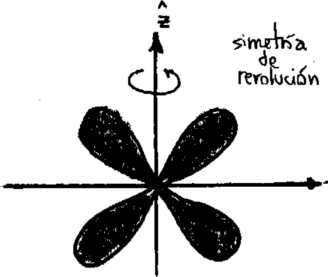
\includegraphics[width=0.4\textwidth]{images/fig_ft1_pot_irrad3.pdf}	 
		\end{center}
		\caption{}
	\end{figure} 
 \item La distribución angular de potencia para la parte cuadrupolar que surge con $\ell=1$ es
	\[
		\left\langle\dtot{P}{\Omega}\right\rangle = \frac{ck^6}{128\pi} Q_0^2 \sin(\theta)^2 
\cos(\theta)^2
	\]
	que es para una fuente con simetría de revolución.
	\[
		\langle\dtot{P}{\Omega}\rangle = \frac{ck^6}{128\pi} |\hat{r} \times \vb{Q} |^2, 
	\]
	donde $\vb{Q}$ es un vector que vale $\hat{n} \cdot \overline{Q}$, o bien indicialmente $n_iQ_{ij}$.
\end{itemize}

\subsection{Radiación a orden $\ell=1$}

\[
	\vb{A} = \frac{1}{cR} \dot{\vb{p}}(t') + \frac{\dot{\vb{m}}(t')}{cR} \times \hat{n} + 
	\frac{1}{6c^2R} {\overline{Q}}(t') \cdot \hat{n}
\]
que es la radiación dipolar eléctrica,  magnética y cuadrupolar eléctrica.

\subsection{Ejemplo de antena}

Sea una pequeña antena de longitud $d$ (ver figura) tal que 
\[
	\vb{J}(\vb{x}') = I \sin( k[d/2 - |z|] ) \delta(x') \delta(y')  \hat{z}
\]
que tiene nodos de la corriente en los extremos. Luego considerando fuente armónica ($A=A(x)\exp(i\omega t)$)
será
\[
	\vb{A}(\vb{x}) = \frac{1}{c} \int_V' \frac{ \vb{J}(\vb{x}') \euler^{ i k |\vb{x}-\vb{x}'| }}
	{ |\vb{x}-\vb{x}'| } dv'
\]

\begin{figure}[htb]
	\begin{center}
	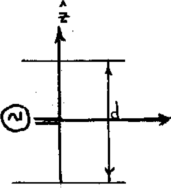
\includegraphics[width=0.3\textwidth]{images/fig_ft1_antena.pdf}	 
	\end{center}
	\caption{}
\end{figure} 

Hacemos algunas aproximaciones geométricas de distancia amparadas en la figura de más abajo.
	\begin{figure}[htb]
		\begin{center}
		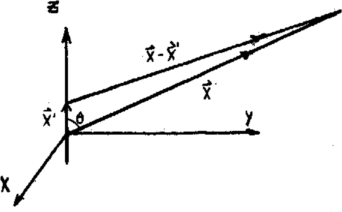
\includegraphics[width=0.4\textwidth]{images/fig_ft1_antena2.pdf}	 
		\end{center}
		\caption{}
	\end{figure} 

Estas aproximaciones son clásicas de los problemas de difracción.
\[
	|\vb{x}-\vb{x}'| = \sqrt{ x^2 + x'^2 - 2xx'\cos(\theta)} =  
	x( 1 - 2x'/x \cos(\theta) + (x'/x)^2)^{1/2} 
\]
y quedándonos a primer orden,
\[
	|\vb{x}-\vb{x}'|\approx x (1 - x'/x \cos(\theta))
\]
de manera que aceptamos una buena aproximación y una bruta,
\[
	|\vb{x}-\vb{x}'| \approx x - x' \cos( \theta ) \qquad \qquad |\vb{x}-\vb{x}'| \approx x
\]
para así escribir
\[
	\approx \frac{1}{|\vb{x}|} \euler^{ikx} \euler^{-ikx'\cos(\theta)}
\]
donde notamos que hemos aproximado de una forma dentro del argumento de la exponencial compleja
y de otra en el denominador de la fracción.

Así, resulta
\[
	\vb{A}(\vb{x}) = \frac{1}{c} \frac{\euler^{ i k x} }{x} \int_V' \vb{J}(\vb{x}') 
		\euler^{ i k x' \cos(\theta) } dv'
\]

Existe condición de contorno que en los extremos la corriente debe ser nula, entonces debe haber nodos
del seno (en $\pm d/2$) y los $d$ posibles son $ n\lambda/2$.
\[
	\vb{A}(\vb{x}) = \hat{z} \frac{2I\euler^{ikx}}{ckx}\left[ \cos( kd/2 \cos(theta) )- 
		\cos( kd/2 ) \right]\frac{1}{\sin(\theta)^2}
\]
entonces 
\[
	\vb{A}(\vb{x}) = A_z \hat{z} \qquad \qquad \vb{A}(\vb{x}) =  A_z\cos(\theta)\hat{\theta} - 
		A_z\sin(\theta) ?
\]
\notamargen{Falta un vegsor}.

Entonces con $ kx' \ll 1$ (longitud de onda larga, $\lambda \gg d $) tenemos
\[
	\left\langle\dtot{P}{\Omega}\right\rangle = \frac{I^2}{2c\pi}\left( \frac{kd}{2} \right)^4 
		\sin(theta)^2
\]
identificando con $|\vb{p}| = Id^2/(2c)$ y este es el primer término multipolar. El paréntesis es muy
chico.
Con media longitud de onda ($kd=\pi$) ($\lambda/2=d$) es
\[
	\left\langle\dtot{P}{\Omega}\right\rangle=\frac{I^2}{2c\pi}\frac{\cos(\pi/2 
	\cos(\theta))^2}{\sin(\theta)^2}
\]
y finalmente para una longitud de onda ($\lambda=2$ y $kd=2\pi$) se tiene 
\[
	\left\langle\dtot{P}{\Omega}\right\rangle=\frac{I^2}{2c\pi} \left[ \frac{ 2\cos(\pi/2 
	\cos(\theta))^2}{\sin(\theta)^2} \right]^2
\]
Las ilustraciones sucesivas de la figura bajo estas líneas dan cuenta de estas diferentes longitudes.

\begin{figure}[htb]
	\begin{center}
	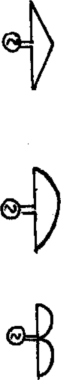
\includegraphics[width=0.1\textwidth]{images/fig_ft1_antena3.pdf}	 
	\end{center}
	\caption{}
\end{figure} 


Como referencia tengamos en cuenta que las expresiones salen de 
\[
	\vb{B}_{rad} = -\frac{1}{c} \hat{n} \times \dot{\vb{A}} = ik \hat{n} \times \vb{A} 
\]
y
\[
	\vb{E}_{rad} = \vb{B}_{rad} \times \hat{n}
\]
Estas equivalencias son para campos de radiación nomás,
\[
	\vb{B}_{rad} = ik \hat{n} \times \vb{A} \qquad \qquad \vb{E}_{rad} = \vb{B}_{rad} \times \hat{n}
\]

% =================================================================================================
\section{Campos de una partícula cargada en movimiento}
% =================================================================================================

Escribimos la densidad de corriente y la densidad de carga según
\[
	\vb{J}(\vb{x}',t') = q\vb{v} \delta[ \vb{x}' - \vb{r}(t')]
\]
\[
	\rho(\vb{x}',t') = q \delta[ \vb{x}' - \vb{r}(t')]
\]
de manera que 
\[
	\vb{A}(\vb{x},t) = \frac{1}{c} \int_{t'}\int_{V'} 
	\frac{ q\vb{v} \delta[ \vb{x}' - \vb{r}(t')] \delta[ t'-t +R/c] }{|\vb{x} -\vb{x}'|} dV' dt'
\]
\[
	\phi(\vb{x},t) = \frac{1}{c} \int_{t'}\int_{V'} 
	\frac{ q \delta[ \vb{x}' - \vb{r}(t')] \delta[ t'-t +R/c] }{|\vb{x} -\vb{x}'|} dV' dt'
\]
donde hemos usado $R\equiv |\vb{x}-\vb{x}'|$ de modo que es $R = R(t')$.
\[
	\vb{A}(\vb{x},t) = \frac{1}{c} \int_v' \frac{ q\vb{v} \delta[ t'-t +R/c] }{|\vb{x} -\vb{r}(t')|} dt' 
	\Rightarrow \vb{A}(\vb{x},t) = \left. \frac{q}{c} \frac{\vb{v}(t')}
	{(1-\hat{n}\cdot{\vb{\beta}})R(t')} \right|_{t'=t-R/c}
\]
\[
	\phi(\vb{x},t) = \frac{1}{c} \int_v' \frac{q \delta[ t'-t +R/c]}{|\vb{x} -\vb{r}(t')|} dt' 
	\Rightarrow \phi(\vb{x},t) = \left. \frac{q}{c} \frac{1}{(1-\hat{n}\cdot{\vb{\beta}})R(t')} 
	\right|_{t'=t-R/c}
\]
cuyas expresiones son los potenciales de Liènard-Wiechert. Hemos usado en las cuentas que 
\[
	\delta[t' - ( t - R(t')/c )] = \frac{1}{\dtot{}{t'}( t' + R(t')/c )} \delta( t-t')
\]
(idea que viene de $\delta f = (1/(df/dx_0)) \delta(x-x_0) $) y que 
\[
	R = |\vb{x}-\vb{x}'| = \sqrt{ x^2 + x'^2 - 2\pe{x}{x'} } \qquad \dtot{R}{t'} = 
	\frac{\dot{\vb{x}'}\cdot(\vb{x}-\vb{x}')}{R} = -\frac{\pe{R}{v}}{R} = -\hat{n}\cdot\vb{v}
\]
\[
	1 + \frac{1}{c} \dtot{R}{t'}  = 1 -\hat{n}\cdot\frac{\vb{v}}{c} = 1 - \hat{n}\cdot\vb{\beta}
\]
según la figura que ilustra bajo estas líneas

\begin{figure}[htb]
	\begin{center}
	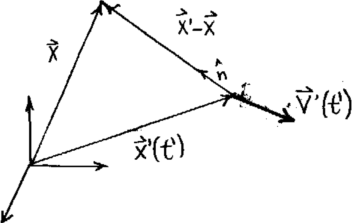
\includegraphics[width=0.4\textwidth]{images/fig_ft1_campo_part_car.pdf}	 
	\end{center}
	\caption{}
\end{figure} 

y como los campos serán 
\[
	\vb{B} = \rotorm{A} \qquad \vb{E} = -\frac{1}{c}\dpar{\vb{A}}{t} - \Nabla\phi
\]
se tiene que 
\[
	\vb{E} = \left. q \frac{ (\hat{n}-\vb{\beta})(1-\beta^2)}{K^3R^2} \right|_{ret} + \left. 
	\frac{q}{c} \frac{\hat{n}\times[ (\hat{n}-\vb{\beta})\times \dot{\vb{\beta}} ]}{K^3R} \right|_{ret}
\]
donde se ve que vale $\vb{B} = \hat{n} \times \vb{E}$ que ya sabíamos para $\vb{E}_{rad}$ y $\vb{B}_{rad}$
y donde $K\equiv 1 - \hat{n}\cdot\vb{\beta} $

De acuerdo a la figura xxxx en $t'$ se produce el campo. Cuando la radiación llega a $\vb{x}$ en tiempo $t$ 
la partícula se halla en $\vb{x}'$ (tiempo $t$), de manera que la moraleja es que $t$ y $t'$ son instantes
de tiempo diferentes en un mismo sistema inercial.

\begin{figure}[htb]
	\begin{center}
	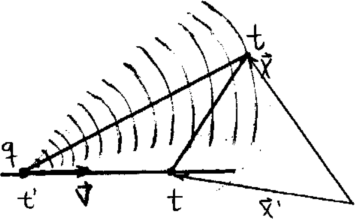
\includegraphics[width=0.4\textwidth]{images/fig_ft1_campo_part_car2.pdf}	 
	\end{center}
	\caption{}
\end{figure} 

Podemos sacar un par de frases importantes ya que 
\begin{itemize}
 \item Si una partícula se mueve con $\vb{v}$ constante puedo pasar a un frame inercial $S'$ donde es 
 $\vb{v}=0$ y entonces $\vb{B}'=0$ de manera que como $\pe{B}{E}=\pe{B'}{E'}=0$ se tiene $\vb{B}\perp\vb{E}$
 en todo frame inercial.
 \item El $\vb{E}_{rad}$ estará dado por el $\vb{E}_a$.
 \item Toda partícula que está acelerada en un frame inercial debe irradiar ondas EM, entonces una partícula
 recorre una circunferencia (en un campo $\vb{B}$) si aceptamos que lo que irradia es despreciable.
\end{itemize}

Sea ahora una partícula $e$ con $|\vb{v}|$ constante, entonces 
\[
	\vb{B}_{bs} = e\frac{\vb{\beta}\times\hat{n}}{\gamma^2k^3R^2} \;\; \text{(Lienard-Wiechert)}
	\qquad \qquad 
	\vb{B}_{bs} = e\frac{\vb{v}\times\hat{n}}{cR^2} \;\; \text{(Biot-Savart)}
\]
y 
\[
	\vb{E}_{v} = e\frac{ \hat{n}- \hat{\beta} }{\gamma^2k^3R^2}
\]
donde vemos que difieren en 
\[
	\frac{1-\beta^2}{(1-\hat{n}\cdot{\vb{\beta}})}
\]


% =================================================================================================
\section{Campo de una carga en movimiento}
% =================================================================================================

El campo de velocidad es 
\[
	\vb{E}_v = e \frac{(\hat{n}-\hat{\beta})}{\gamma^2(1-\hat{n}\cdot\vb{\beta})^3R^2} =
		e \left[ \frac{\vb{R}-R\vb{\beta}}{\gamma^2(1-\hat{n}\cdot\vb{\beta})^3R^2} \right]
\]
referidas las magnitudes a la figura XXXX.

\begin{figure}[htb]
	\begin{center}
	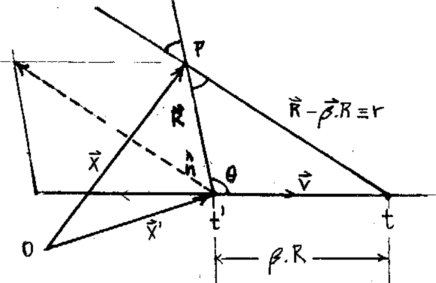
\includegraphics[width=0.4\textwidth]{images/fig_ft1_campo_carga_mov2.pdf}	 
	\end{center}
	\caption{}
\end{figure} 

\[
	|\vb{E}_v| = e\frac{\sqrt{ R^2 + \beta^2 R^2 - 2R^2 \beta \cos(\theta)}}
		{\gamma^2( 1 - \vb{R}\cdot\vb{\beta}/R)^3 R^3} =
		e\frac{\sqrt{ 1 + \beta^2 - 2 \beta \cos(\theta)}}
		{\gamma^2( 1 - \beta \cos(\theta))^3 R^2}
\]
entonces como $\cos(\theta) = \beta$
\[
	\dtot{ |\vb{E}_v| }{\theta}= 0
\]
siendo los extremos $\theta=0,\pi$ que representan un movimiento hacia adelante o hacia atrás.
\[
	|\vb{E}_v(\cos(\theta) = \beta)| = \frac{e\gamma}{r^2}
\]
\[
	|\vb{E}_v(\cos(\theta) = 1)| = \frac{e (1+\beta^2-2\beta)^2}{R^2(1-\beta^2)^{-1}(1-\beta)^3}
\]
\[
	|\vb{E}_v^{(\theta = 1)}| = \frac{e }{R^2(1-\beta^2)^2 \gamma^2} = \frac{e}{r^2 \gamma^2}
\]
puesto que es $r=R(1-\beta)$. Vemos que es similar al campo estático pero con un factor corrector.

Campo de aceleración, es
\[
	\vb{E}_a = \frac{e}{c} \frac{ \hat{n} \times [ (\hat{n}-\vb{\beta})\times \dot{\vb{\beta}} ]}{K^3 R} 
		\approx \frac{e}{c} \frac{ \hat{n} \times ( \hat{n} \times \dot{\vb{\beta}})}{K^3 R} 
		= \frac{e}{c} \frac{}{K^3 R}
\]
donde usamos que $v/c \ll 1$ y por ende $ 1 - \hat{n}\cdot\vb{\beta}\approx 1$ entonces es 
\[
	\hat{n} \cdot \hat{\beta} \approx \hat{n}
\]

\begin{figure}[htb]
	\begin{center}
	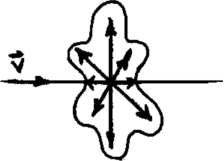
\includegraphics[width=0.4\textwidth]{images/fig_ft1_campo_carga_mov.pdf}	 
	\end{center}
	\caption{}
\end{figure}

% =================================================================================================
\section{Cálculo de potencia irradiada}
% =================================================================================================

\begin{figure}[htb]
	\begin{center}
	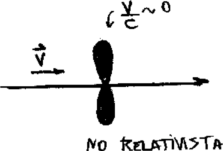
\includegraphics[width=0.4\textwidth]{images/fig_ft1_frenado2.pdf}	 
	\end{center}
	\caption{}
\end{figure} 

\begin{figure}[htb]
	\begin{center}
	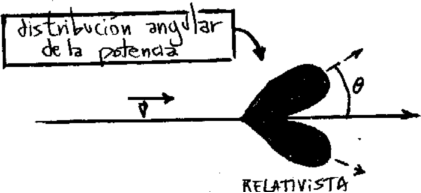
\includegraphics[width=0.4\textwidth]{images/fig_ft1_frenado3.pdf}	 
	\end{center}
	\caption{}
\end{figure} 

% =================================================================================================
\section{Frenado magnético}
% =================================================================================================

\begin{figure}[htb]
	\begin{center}
	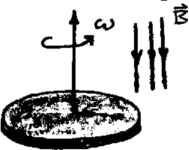
\includegraphics[width=0.4\textwidth]{images/fig_ft1_frenado.pdf}	 
	\end{center}
	\caption{}
\end{figure} 

% =================================================================================================
\subsection{Esponja electromagnética}
% =================================================================================================

\begin{figure}[htb]
	\begin{center}
	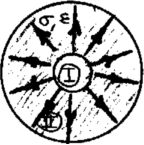
\includegraphics[width=0.4\textwidth]{images/fig_ft1_esponja.pdf}	 
	\end{center}
	\caption{}
\end{figure} 

% \bibliographystyle{CBFT-apa-good}	% (uses file "apa-good.bst")
% \bibliography{CBFT.Referencias} % La base de datos bibliográfica

\end{document}

	
% 	\input{FT1.c9}
	
	%###########################################################################
	%		FIN DE LOS CAPITULOS DEL CURSO
	%###########################################################################
	
	%##########################	INDICE	########################################
	
% 	La bibliografía se activará al final cuando se comente la de cada chapter
	
% 	\bibliographystyle{plain}	
%	\bibliographystyle{CBFT-apa-good} % (uses file "apa-good.bst")
% 	\bibliography{CBFT.Referencias} % La base de datos bibliográfica
	
	
	
	\end{document}